\chapter{The Large Hadron Collider}\label{thelhc}
%
%
The Large Hadron Collider (\acrshort{LHC}) is the world's largest particle accelerator, designed to store and accelerate proton and \lead beams at unprecedented energies of 7$\,Z\,$TeV. The LHC is a synchrotron of 26.7\,km length, installed in the underground tunnel built for the Large Electron Positron Collider (LEP) at the CERN\footnote{Centre Europ\'{e}en pour la Recherche Nucl\'{e}aire.} research center near to Geneva, Switzerland. With the Relativistic Heavy-Ion Collider (RHIC) at the Brookhaven National Laboratory and the former CERN Intersecting Storage Rings (ISR)~\cite{ISRref}, it is one of the three heavy-ion colliders ever built and operated~\cite{Fischer2014}. In the first operational period (Run 1), the LHC reached energies up to 4$\,Z\,$TeV with proton and \lead beams. With the collected data, the discovery of the long sought Higgs boson was announced in July 2012~\cite{higgs:ATLAS,higgs:CMS}. After a phase of machine and detector upgrades from 2013 to 2015, the LHC restarted into \mbox{Run 2} and accelerated proton beams to the unprecedented energy of $6.5\,$TeV and \lead beams to $6.37\,Z\,$TeV.
%

In this chapter the LHC is presented with the sub-systems relevant for the development of heavy-ion collimation simulation tools presented later-on. Particular emphasis is given to the LHC collimation system and the interaction of particles with the collimator material, which has an important influence on the efficiency of the collimation system.

%
\section{The CERN Accelerator Complex}
%
  \begin{figure}[t]
    \centering
    \includegraphics[width=0.85\textwidth]{pictures/14052201.png}
    \caption{ The CERN Accelerator Complex~\cite{Christiane:1260465}.}  
    \label{pic:14052201}
  \end{figure}
%
The LHC is a high-energy synchrotron operated at the end of a complex chain of injectors which pre-accelerate and prepare the beam for its requirements. The ensemble of accelerators currently operated at CERN is referred to as the CERN accelerator complex. It is schematically illustrated in Fig.~\ref{pic:14052201}. 

The LHC injector chain starts with two different ion sources, respectively delivering proton or heavy-ion beams. The generation of proton beam starts at a hydrogen ion source feeding the linear accelerator LINAC2, in which the proton beam is accelerated to a momentum\footnote{For clarity, in this chapter the momentum is given in natural units. All given momenta shall correspond to the correct unit of eV$/c$. Furthermore, the energies for the non fully stripped ions are given in terms of momentum per nucleon, while for the fully stripped ions, the general convention of using the momentum per charge is followed.} of 50~MeV and injected into the Proton Synchrotron Booster (PSB). This synchrotron accelerates the beam to 1.4~GeV, the injection energy of the Proton Synchrotron (PS) which provides acceleration up to 25~GeV. After the subsequent injection into the Super Proton Synchrotron (SPS), the beams are brought to 450~GeV, the injection energy of the LHC~\citedr. 
%

Heavy-ion beams start from the ion source upstream of the linear accelerator LINAC3. The ions are generated from a block of lead, enriched with the isotope $^{208}$Pb, by means of an Electron Cyclotron Resonance Source~\cite{CERN-2004-003-V1}. The source delivers ions at a momentum of 2.5\,keV/$A$, which are sent to a spectrometer in order to extract the desired Pb$^{27+}$ charge state. After the filtering, a multi-stage RF system accelerates the selected ion species to a momentum of $4.2\,$MeV/$A$. The following 300~nm thick stripper foil removes more electrons, such that an ion beam of Pb$^{53+}$ is extracted from LINAC3 and transferred to the circular accelerator LEIR (Low Energy Ion Ring). In the latter, the ion beams are cooled, e.g. the transverse emittance is reduced by an adiabatic process using electron scattering. In parallel, the beam is accelerated to a momentum of 72$\,$keV$/A$ at which it is extracted and transferred into the PS. In this machine, the ion bunches are re-shaped, accelerated to a momentum of 5.9$\,$GeV$/A$ and finally sent to the SPS. Another stripper foil in the transfer line between PS and SPS removes the remaining electrons, such that the ion arriving at the SPS is \lead. The SPS provides the acceleration to the energy of $450\,Z\,$GeV at which the beams are injected into the LHC~\citedr.


\section{LHC Design and Performance}
\subsection{Global Layout}
%
The global LHC layout is illustrated in \figref{pic:15032201}. The LHC houses eight straight sections (also called insertion regions, IR). Four of them host the main experiments ATLAS~\cite{ATLASref01}, \mbox{ALICE}~\cite{ALICEref01}, CMS~\cite{CMSref01} and LHCb~\cite{LHCbref01}. The remaining four IRs provide operational functionalities, namely betatron and momentum cleaning in IR3 and IR7 (see \chapref{chap:3}), acceleration in IR4 and the beam dump in IR6. The straight insertion regions are separated by the LHC arc regions. In the latter, a periodic array of superconducting dipole magnets and superconducting quadrupole magnets provides the guiding and focusing forces required to transport the beam between the IRs. 

%
%


\begin{figure}[b]
  \centering
  \begin{tikzpicture}
    \node[anchor=south west,inner sep=0] (image) at (0,0) {\includegraphics[width=0.70\linewidth]{pictures/15092509.pdf}};

  % \draw[help lines,step=.2] (0,0) grid (16.0,9.0);
  % \draw[help lines,line width=.6pt,step=1] (0,0) grid (16.0,9.0);
  % \foreach \x in {0,1,2,3,4,5,6,7,8,9,10,11,12,13,14,15,16}
  %      \node[anchor=north] at (\x,-0.1) {\x};
  % \foreach \y in {0,1,2,3,4,5,6,7,8,9}
  %     \node[anchor=east] at (-0.2,\y) {\y};

      \filldraw[fill=white, draw=white] (3,1) rectangle (9,1.25);
    %\node [draw,rotate=90,x={(image.south east)},y={(image.north west)}]                   at (0.50,0.50)    {text0};
    %\node [draw,rotate=0 ,x={(image.south east)},y={(image.north west)}]                   at (0.22,0.96)    {text1};
    %\node [draw,rotate=0 ,x={(image.south east)},y={(image.north west)},anchor=west]       at (0.22,0.80)    {text2};
    \draw[<->,color=black,thick]             (3.95,1.0) -- (7.35,1.0);
  \end{tikzpicture}
  \caption{The layout of the LHC. Based upon \cite{Bruning2012705,CERN-2004-003-V1}.}  
  \label{pic:15032201}
  \end{figure}




% \begin{figure}[b]
%   \centering
%   \includegraphics[width=0.7\textwidth]{pictures/15092509.pdf}
%   \caption{The layout of the LHC. Based upon \cite{Bruning2012705,CERN-2004-003-V1}.}  
%   \label{pic:15032201}
%   %/home/phermes/Dropbox/codes/latex/150305_eps2pgf/test.pdf
% \end{figure}

\subsection{Naming Conventions}

The two counter-rotating LHC beams are called Beam 1 (B1), which circulates in clockwise direction and Beam 2 (B2), which circulates in counter-clockwise direction. The position $s$ in the LHC is measured from IP1 in clockwise direction. 

Each element of the LHC is associated with a cell number, indicating the number of quadrupoles between the closest IP and the respective location. For example the name MQY.4L5.B1 denotes a quadrupole of the MQY type (see \cite{CERN-2004-003-V1}) in cell 4 left of IP5 for Beam 1. 



\subsection{Optics and Insertion Region Layout}

%IR should be explained in previous section


%
\begin{figure}[b]  
    \centering
    \includegraphics[width=0.9\textwidth]{pictures/16051203.pdf}
    \caption{Optical functions of B1 at the experimental insertion IR5 with $\beta^*=1\,$m for a flat machine (no separation or crossing bump).}  
    \label{pic:16051202}
    %/home/phermes/Dropbox/PhD/pictures/160403_optics/IR5.pdf
\end{figure}
%
The schematic layout of the experimental insertion regions is shown together with the $\beta$ functions in \figref{pic:16051202}. Downstream of the main arcs (1) in which the beams are transported between the IRs, the dispersion suppressor (DS) region (2) serves the purpose of reducing the periodic dispersion function. This is reached by means of a missing dipole structure, in which one of the three dipoles of the regular arc lattice is omitted~\citedr. In between the surrounding DS regions, the IR is free of the main dipoles and therefore straight. After the DS, the matching section (3) adjusts the $\beta$ functions to the requirements of the following sections. The separation/recombination dipoles (4) and (5) guide the beams from the separated beam pipes into a common beam pipe. The superconducting triplet magnets (6) provide the final focusing for the  interaction point (7) (IP), where the beams are brought into collision.

The experiments ATLAS and CMS demand for the highest possible luminosity in order to gain enough statistics for the study of rare processes (see \chapref{chap:lumi}). As discussed later, the luminosity is inversely proportional to the $\beta$ value at the IP (denoted as $\beta^*$), thus the optics is optimized to minimize the $\beta^*$ value. Following Liouville's theorem, small $\beta$ functions imply a large divergence (large $\alpha$ function) at the IP and, due to the absence of magnets between IP and triplet, the $\beta$ functions (and associated with it the beam size) at the superconducting triplets increase with smaller $\beta^*$. The dimensions of the triplet aperture therefore impose a lower limit on the achievable $\beta^*$. The transition to the smallest $\beta^*$ settings (referred to as squeeze) is performed either at top energy or during the last part of the energy ramp (see \chapref{chap:lhccycle}), because the beam sizes decrease with energy due to the adiabatic damping. At injection energy, the optics in IR1 and IR5 are set to $\beta^*=11\,$m while IP2 and IP8 are set to $\beta^*=10\,$m. A summary of the minimum $\beta^*$ values achieved at top energy during the past LHC runs is given in \tabref{tab:betastar}. 
%
%
\begin{table}[t]
\centering
\caption{Minimum $\beta^*$ values in LHC operation compared to the design values.}
\label{tab:betastar}
\begin{tabular}{cccccc}
Configuration & Species & \begin{tabular}[c]{@{}c@{}}$\beta^*$ [m]\\
IP1/IP5\end{tabular} & \begin{tabular}[c]{@{}c@{}}$\beta^*$ [m]\\
IP2\end{tabular} & \begin{tabular}[c]{@{}c@{}}$\beta^*$ [m]  \\ IP8
\end{tabular}  & Energy [$Z\,$TeV] \\ \toprule
%
Design & p & 0.55 & 10.0 & 10.0 & 7.0 \\
2011 & p & 1.0 & 10.0 & 3.0  & 3.5   \\
2012 & p & 0.6 & 10.0 & 3.0  & 4.0   \\
2015 & p & 0.8 & 10.0 & 3.0  & 6.5   \\
2016 & p & 0.4 & 10.0 & 3.0   & 6.5  \\ \midrule
Design & Pb & 0.5 & 0.5 & 10.0  & 7.0   \\
2011 & Pb & 1.0 & 1.0 & 3.0   & 3.5    \\
2013 & p-Pb & 0.8 & 0.8 & 2.0 & 4.0  \\
2015 & Pb & 0.8 & 0.8 & 3.0    & 6.37   \\ \bottomrule
%
\end{tabular}
\end{table}
%
% table: proton and ion runs, beta*


In the central part of the experimental insertions, both beams are moving in a common vacuum pipe to bring them into collision at the IP. In order to avoid unwanted collisions of the counter-rotating beams, a separation bump is applied when collisions are not supposed to occur. In addition, a crossing angle avoids secondary collisions at parasitic bunch encounters when the beams are brought into collision.  The crossing and separation bumps in the high luminosity insertions are orthogonal to each other. Both bumps are shown for the example of IR5 in \figref{pic:16051204}. The IRs without experiments are not equipped with triplet magnets and the optics is adjusted for the purpose of the installed hardware. The layout, functionality and optics of the collimation insertion regions are discussed in \chapref{chap:3}. 

% The closed orbit in the experimental insertions is in general at the center of the beam pipe. Exceptions are  In these regions, the beam orbits are not in the center of the beam pipe to avoid unwanted collisions of the counter-rotating beams. A seperation bump is applied during all phases except when the beams should collide in the IP. The seperation bump is collapsed to establish collisions~\citedr. 

% Depending on the bunch spacing, multiple encounters of the two counter-rotating beams may be localized in the common beam pipe. The application of a crossing bump prevents from parasitic collisions at these secondary bunch encounters.


%
%
%
\begin{figure}[htbp]  
    \centering
    \includegraphics[width=0.7\textwidth]{pictures/16051204.pdf}
    \caption{Separation and crossing bumps in IR5 during the 2011 heavy-ion run with $\beta^*=1\,$m.}  
    \label{pic:16051204}
    %/home/phermes/Dropbox/PhD/pictures/160403_optics/bumps.pdf
\end{figure}
%
%


\subsection{Operational Cycle} \label{chap:lhccycle}
% 
\begin{figure}[b]  
    \centering
    \includegraphics[width=0.8\textwidth]{pictures/16051201.pdf}
    \caption{Beam energy, intensity and $\beta^*$ during the LHC cycle.}  
    \label{pic:16040801}
    %/home/phermes/Dropbox/PhD/pictures/160408_cycle/cycle.pdf
\end{figure}
%

The LHC operational cycle is a defined protocol which ensures safe operation and avoids uncertainties of the magnetic fields which could possibly arise from hysteresis.  In \figref{pic:16040801}, the LHC cycle is illustrated for an ideal \lead physics fill in the 2015 heavy-ion run. 

In the \textit{injection} mode (1) at a beam energy of 450$\,Z\,$GeV, the machine is ready to receive particle bunches from the injectors. The beams are not squeezed in this configuration, to obey the tight aperture restrictions. The optics in the injection insertions IR2 and IR8 are designed to optimize the phase advance between the injection septum the injection protection collimators. 

Once the LHC is filled with beam, the mode is changed to \textit{prepare ramp} (2), in which the injection protection collimators are retracted to allow for the following \textit{ramp} (3), the acceleration to top energy. During the ramp, power converters, RF and collimators are synchronously adjusted to follow the beam energy and the decreasing beam size.

%\newpage
After the ramp, the \textit{squeeze} (4) is a stepwise optical sequence in which the $\beta^*$ value in the high luminosity IRs is smoothly reduced to the final value for collision. Finally, the beam mode changes to \textit{adjust} (5), in which the separation bump is collapsed and small additional bumps are introduced to correct for deviations in the closed orbit and maximize the luminosity in the experiments. Once the collisions in the experimental IRs are established, the beam mode is referred to as \textit{stable beams} (6). 
The stable beam mode is maintained for several hours until the luminosity has decreased below a certain level. Then the beams are intentionally \mbox{dumped (7)}. The magnet currents are then reduced (\textit{ramp down}, (7)) to a level below the injection level to eliminate hysteresis effects before the following injection mode. Note that for heavy-ion operation in 2015, the last part of the cycle was carried over from the previous proton run in which the protons had larger rigidities. The ramp down therefore included an increase of the magnet currents from the operational setting at 6.37$\,Z\,$TeV to the proton setting at 6.5$\,$TeV.

In 2016, the formerly distinct steps of ramp and squeeze have been merged to reduce the time to set up the stable beams configuration and thus increase the integrated luminosity. This combined ramp and squeeze~\cite{IPAC12:MOPPC016} synchronously accelerates the beams to 6.5~TeV and reduces the $\beta$ functions at IP1 and IP5 to $\beta^*=3\,$m.



\subsection{Luminosity} \label{chap:lumi}

An important measure for the performance of a collider is the luminosity. The instantaneous luminosity $\mathcal{L}(t)$ is the proportionality between the cross section $\sigma_p$ of a physical process and the expected event rate $\frac{\mathrm{d}N_p}{\mathrm{d}t}$ in a given machine configuration~\cite{wiedemann1999particle}:
%
\begin{align}
  \frac{\mathrm{d}N_p (t)}{\mathrm{d}t} = \mathcal{L}(t) \, \sigma_p \, . \label{eq:eventrate}
\end{align}
%
The luminosity is proportional to the number of bunches $n_B$, the square of the number of particles per bunch $N_B$, the revolution frequency in the machine $f_\text{rev}$, the relativistic $\gamma$ and inversely proportional to the $\beta^*$ value and the normalized emittance\footnote{This formula applies for round beams; e.g. when $\beta^*$ and the emittance $\epsilon$ are identical in both planes for both beams.}:
\begin{align}
  \mathcal{L} = \frac{n_B N_B^2 f_\text{rev} \gamma}{4 \pi \epsilon_N \beta^*} \, F \, . \label{eq:lumi}
\end{align}
%
The additional factor $F$ takes into account for the luminosity reduction due to the fact that the colliding bunches are not fully overlapping when a crossing angle $\theta_C$ is applied. 

%\newpage
The correction factor depends on the longitudinal RMS beam size $\sigma_l$, the transverse beam size at the IP \mbox{($\sigma_x=\sigma_y=\sigma^*$)} and the crossing angle as follows~\cite{proceedingsCAS:herr}:
%
\begin{align}
  F = \frac{1}{\sqrt{1 + \left( \frac{\theta_C \, \sigma_l }{2 \, \sigma^*}  \right)^2 }} \, .
%  F = \frac{1}{\sqrt{1+\left(\frac{\sigma^*}{\sigma_l} \, \tan \frac{\theta}{2} \right)}} \, \frac{1}{\sqrt{1+\left(\frac{\sigma_l}{\sigma^*} \, \tan \frac{\theta}{2} \right)}} \,.
\end{align}
%
For heavy-ion collisions, it is important to measure the number of colliding nucleons, rather than nuclei. This is especially true if the collider produces asymmetric collisions (e.g. p-Pb collisions) or if the luminosity with different isotopes should be compared. The nucleon-nucleon luminosity $\mathcal{L}_\text{NN}$ is defined as
%
\begin{align}
  \mathcal{L}_\text{NN} = A_1 \, A_2 \, \mathcal{L} \, ,
\end{align}
where $A_1$ and $A_2$ are the nuclear mass numbers of the colliding nuclei.

Following \eqref{eq:lumi}, the luminosity is measured in the unit cm$^{-2}\,$s$^{-1}$, which corresponds to $10^{24}\,\text{b}^{-1} \, \text{s}^{-1}$. The latter expression in combination with the definition given in \eqref{eq:eventrate} elegantly illustrates the dependence of the number of expected events with a given cross section (measured in barns) per time unit. Even more information on the performance of the accelerator can therefore be obtained if the instantaneous luminosity is integrated over the total time $T$ the machine is operated in stable beams. This quantity is referred to as the integrated luminosity:
%
\begin{align}
  \mathcal{L}^\text{int} = \int_{0}^T \mathcal{L}(t) \, \mathrm{d} t \, .
\end{align} 
%
Obviously, it is of great interest to maximize the integrated luminosity, in order to allow the study of rare events. This can be done either by increasing the instantaneous luminosity (if not restricted by the experiments) or by optimizing the operational cycle of the machine, to maximize the time the machine can be operated in the stable beams mode.

%\input{pictures/16070312.tex}
  % #PHTHESIS FILE ORIGIN
  %/home/phermes/workspace/tikz/drawing.tex

%
The instantaneous luminosity can be increased if smaller $\beta^*$ values are applied, the emittance is reduced, the stored beam intensity is increased or if the luminosity reduction factor is enlarged. While the achievable emittance, number of bunches and bunch intensity depend strongly on the performance of the LHC injectors, the $\beta^*$ value is imposed to a lower limit due to aperture restrictions in the triplet magnets~\cite{PhysRevSTAB.18.061001}. The geometrical luminosity reduction factor $F$ could be improved by reducing the crossing angle, which has a lower limit imposed by the long range beam-beam interaction.
%

% From the hardware side, the latter can possibly be improved by deciated RF cavities, the crab cavities~\cite{Calaga:Chamonix12}. As shown in \figref{pic:cc} they tilt the colliding bunches to increase their overlap at the collision point. This approach reduces the effective crossing angle and so improves the factor $F$. 
 






\subsection{LHC Performance in Previous Runs} \label{chap:lhccycle}
%

In this section, the LHC program so far is briefly introduced. The achieved beam parameters in operation with p-p, p-Pb and Pb-Pb are summarized and compared to the design parameters \tabref{tab:lhc_protonsparams} and \tabref{tab:lhc_parameters}.

\subsubsection{Proton Beams}

\begin{table*}[b]
\centering
\caption{Comparison of the LHC design beam parameters for proton beams~\cite{Alemany-Fernandez:1631030,HB2016:MOAM5P50}. The quantity $n_B$ describes the number of bunches, $E_s$ the total stored beam energy and $N_B$ the number of particles per bunch. The data for 2016 is as of July 2016 and may be subject to change.}
\label{tab:lhc_protonsparams}
 
\begin{tabular}{cc|c|ccccc}
\multicolumn{2}{c|}{} &  \multicolumn{1}{c|}{Nominal} & \multicolumn{4}{c}{Achieved in the LHC} \\ \toprule

\multicolumn{2}{c|}{Year}     &         & 2010   & 2011   & 2012   & 2015   & 2016                            \\ \midrule
$E$                & [TeV]    & 7       & 3.5    & 3.5    & 4.0    & 6.5    & 6.5                             \\
$\gamma$           &          & 7460.5  & 3730.3 & 3730.3 & 4263.2 & 6927.6 & 6927.6                          \\
$n_B$              &          & 2808    & 368    & 1380   & 1380   & 2244   & 2220                            \\
$N_B$            & [$10^{11}$] & 1.15    & 1.0    & 1.3    & 1.5    & 1.1    & 1.1                             \\
$\epsilon_N$  & [\mum$\,$rad] & 3.75    & 2.6    & 2.4    & 2.4    & 3.5    & 3.4                             \\ 
$E_s$ &[MJ]                   & 362     & 23     & 112    & 143    & 277    & 266                             \\
$\mathcal{L}_\text{peak}$ &[$10^{34}\,$cm$^{-2}\,$s$^{-1}$] 
                              & 1.0     & 0.021  & 0.35   & 0.77   & 0.51   & 1.2                            \\
$\mathcal{L}^\text{int}$ & [fb$^{-1}$]
                              &         & 0.0048 & 5.5    & 22.8   & 4.2    & 8.1                             \\ \bottomrule
\end{tabular}
\end{table*}





The LHC proton program started with the first data taking phase in 2010. In this first operational period the LHC was operated with small beam intensities at 3.5\,TeV, half the design energy. With the operational experience gained, the stored beam intensity could be increased by almost one order of magnitude in 2011, and a significant amount of integrated luminosity was collected. The 2012 proton operation was fully dedicated to luminosity production and the integrated luminosity could be doubled with respect to the precedent year. In this year the maximum  particle energy was increased to 4\,TeV~\cite{IPAC16:WEOCA01}.

At the beginning of 2013, the operation of the LHC stopped for long shutdown 1 (LS1), a consolidation and upgrade phase with the main purpose of consolidating the superconducting splices in order to reach proton momenta of 6.5\,TeV to 7.0\,TeV~\cite{IPAC13:MOZB202}.
After a successful restart in 2015, the LHC was operated at an unprecedented proton energy of 6.5\,TeV. In the following year, the LHC operated the first time at nominal luminosity due to the reduced $\beta^*$ value and increased bunch intensity.



\subsubsection{Heavy-Ion Beams}


\begin{table*}[b]
\centering
\caption{Comparison of the LHC design beam parameters for heavy-ion beams compared to the values achieved in the previous LHC heavy-ion runs~\cite{CERN-2004-003-V1,pPbref01,jowett-RLIUP13,PbPbref01,Jowett:1492972}. The parameters given for p-Pb operation refer to the \lead beam. The integrated luminosity is given in terms of nucleon-nucleon encounters~\cite{IPAC16:TUPMW027}.}
\label{tab:lhc_parameters}
 
\begin{tabular}{cc|c|cccc}
\multicolumn{2}{c|}{} &  \multicolumn{1}{c|}{Nominal} & \multicolumn{4}{c}{Achieved in the LHC} \\ \toprule

\multicolumn{2}{c|}{Year}          &       & 2010  & 2011 & 2013 & 2015 \\% \midrule
\multicolumn{2}{c|}{Species}       & Pb-Pb & Pb-Pb & \multicolumn{1}{c}{Pb-Pb} & p-Pb & \multicolumn{1}{c}{Pb-Pb} \\ \midrule
$E$          & {[}TeV{]}     & 7$\,Z$ & 3.5$\,Z$ & 3.5$\, Z$ & 4.0$\, Z$ & 6.37$\,Z$\\

$\gamma$     &               & 2963.5 & 1481.8 & 1481.8 & 1693.4 & 2696.8\\

$n_B$        &                & 592 & 137 & 358 & 338 & 518\\

$N_B$        & {[}$10^8${]}   & 0.7 & 1.12 & $1.20 \pm 0.25$ & $1.40\pm0.27$ & $2.2\pm0.3$\\

$\epsilon_N$ & {[}$\mu$m$\,$rad{]}  & 1.5 & 2.0 & $1.7\pm0.2$ & - & $1.50\pm0.15$ \\

$E_s$ &{[}MJ{]}  & 3.81 & 0.71 & 1.98$\pm$0.42 & 2.18$\pm$ 0.42 & 9.54$\pm$1.30\\

$\mathcal{L}_\text{peak}$ &[$10^{27}\,$cm$^{-2}\,$s$^{-1}$]  & \begin{tabular}[c]{@{}l@{}}1 (Pb-Pb)\\ 115(p-Pb)\end{tabular} & 0.03 & 0.5 & 110 & 3.0\\ 
$\mathcal{L}^\text{int}_\text{NN}$ & [pb$^{-1}$]   &         &  0.4  &  19.9   &  20.2  &   76.0                              \\
\bottomrule
\end{tabular}
\end{table*}

The first LHC run with heavy ions took place in 2010, in which mostly operational experience at 3.5\,$Z\,$TeV was collected. The second heavy-ion run in late 2011 was carried out at 3.5\,$Z$\,TeV and delivered half the design luminosity~\cite{PbPbref01}. In 2013 a mixed particle mode was established, in which protons were collided with \lead ions at 4$\,Z\,$TeV~\cite{pPbref01}. 

The 2015 operational period with heavy ions started with a reference proton run at 2.51$\,$TeV per beam in order to obtain the same center of mass energy as in the p-Pb run of 2013. For the same reason, the ensuing Pb-Pb operation was carried out at an energy of $6.37\,Z\,$TeV, instead of the 6.5$\,Z\,$TeV which would have been possible after the precedent proton operation at equivalent rigidity~\cite{IPAC16:TUPMW027}. This allows the experiments to compare data at the same center of mass energy for three different collision types: p-p, p-Pb and Pb-Pb. In the 2015 Pb-Pb running period, the LHC exceeded the design value of the stored \lead beam energy more than twice, due to the better-than-nominal performance of the LHC injectors. The bunch intensity has tripled with respect to the design value. This remarkable performance led to an excess of the design luminosity by a factor three~\cite{IPAC16:TUPMW027}.


\subsection{High Luminosity LHC} \label{chap:introhl}



For the future of the LHC, a drastic increase of the luminosity is foreseen for both proton and heavy-ion operation, to improve the potential for discoveries. The future LHC configuration with increased luminosity is referred to as High Luminosity LHC (HL-LHC)~\cite{HLDR,hllhc:asdhep}.

An essential keystone for this objective is the increase of the bunch intensity and, for heavy ions, the possible number of bunches that can be stored in the machine. This is made possible by the LHC injectors upgrade (LIU)~\cite{IPAC11:WEPS017,IPAC2015:THPF093}, a modification of the injector chain with hardware upgrades and even the replacement of LINAC2 by a new H$^-$ accelerator LINAC4~\cite{IPAC2015:THPF093}. The schedule to reach the HL-LHC parameters foresees a stepwise luminosity increase in which double of the design luminosity shall be reached after LS2 in 2020~\cite{hllhc:asdhep}.




The current baseline envisages the commissioning of the High Luminosity LHC (HL-LHC) adapted for a peak luminosity with proton beams more than seven times the LHC design value as of 2025. To allow for this increase, extensive hardware upgrades in IR1 and IR5 are required, one of them being the installation of crab cavities~\cite{HLDR}. Furthermore, the replacement of several magnets is required. The inner magnets in IR1 and IR5 (including the triplet magnets, separation/recombination dipoles and Q4 and Q5) are replaced by new magnets with a larger aperture to allow for smaller $\beta^*$ values~\cite{HLDR}. Presently, it is foreseen to apply $\beta^*=0.15\,$cm for protons and $\beta^*=0.48\,$m for heavy-ion beams in IR1 and IR5. Further upgrades concern the LHC collimation system, which is discussed in \chapref{hl:coll}.


%
	\begin{table}[b]
		\centering
		\caption{Comparison of heavy-ion beam parameters: design parameters~\cite{CERN-2004-003-V1}, achieved in the 2015 heavy-ion run, envisaged parameters for LIU and HL-LHC~\cite{jowett:private}. The baseline for the heavy-ion species is \lead for all cases.}
		\label{tab:LIU_HL_Parameters}
		
		\begin{tabular}{cccccccc}
			\toprule
			                        & $E$             & $n_B$   & $\epsilon_N$  & $N_B$             & $E_s$     \\ %\midrule
			                        & {[}$Z$ TeV{]}	  &         &  $\mu$m rad   &  [$10^7$ ions]     & [MJ]             \\ \midrule
			Design                  & 7.0             & 592     & 3.75 & $7$               & 3.81             \\
			2015                    & 6.37            & 518     & 1.5$\pm 0.15$ & 22$\pm3$              & 9.54$\pm1.30$             \\
			LIU baseline            & 7.0             & 1152    & 1.2  & $17$              & 18.0             \\
			HL-LHC request          & 7.0             & 1248    & 1.3 & $21 $             & 24.1             \\ \bottomrule
		\end{tabular}
	\end{table}
%


Optimistic estimates for the heavy-ion beam parameters after the LIU and HL-LHC upgrade are compared to the design values and those achieved in 2015 in \tabref{tab:LIU_HL_Parameters}. 






\section{The LHC Magnets}

Many different types of magnets provide the guiding and confining forces required for the operation of the LHC. Except the magnets in the inner part of the experimental insertions, where the two beams are brought into collision, the LHC magnets are double-bore magnets in which both beams circulate in separated beam pipes, as shown in \figref{pic:16070405}. In this section, the superconducting LHC main dipoles and quadrupoles are briefly introduced and their superconducting properties are discussed. The risk of beam induced quenches (transition from superconducting to normal conducting state) for these magnets is one of the motivations for the LHC collimation system explained in the following section. More detailed information can be found in \citedr.

\begin{figure}[b]
  \centering
  \begin{tikzpicture}
    \node[anchor=south west,inner sep=0] (image) at (0,0) {\includegraphics[width=0.6\linewidth]{pictures/16070405.png}};
    %\node [draw,rotate=90,x={(image.south east)},y={(image.north west)}]                   at (0.50,0.50)    {text0};
    %\node [draw,rotate=0 ,x={(image.south east)},y={(image.north west)}]                   at (0.22,0.96)    {text1};
    %\node [draw,rotate=0 ,x={(image.south east)},y={(image.north west)},anchor=west]       at (0.22,0.80)    {text2};
    %\draw[->,color=black,thick,x={(image.south east)},y={(image.north west)}]             (0.42,0.22) -- (0.37,0.23);
  \end{tikzpicture}
  \caption{Cross section of the LHC double bore main dipole magnet~\cite{Valeriane:843195}.}  
  \label{pic:16070405}
  %/home/phermes/Desktop/dipole.png
  \end{figure}


\subsection{Main Dipoles}

The 1232 superconducting LHC main dipoles (MB) are horizontal bending magnets of 14.3~m magnetic length, capable of delivering a maximum magnetic field of 8.3~T. They are designed to provide a bending radius of $\rho_0=\frac{1}{h_x} = 2804~\text{m}$, yielding a maximum particle energy of $7\,Z\,$TeV. To keep the NbTi coils in a superconducting state, they are cooled with liquid helium to be operated at a temperature of 1.9~K. More information on the superconducting LHC dipoles can be found in \citedr.
%
\subsection{Quadrupoles}
The LHC is equipped with many different quadrupoles to provide the focusing required to confine the beams in the LHC arcs and prepare their optical functions for the collision in the IPs. Depending on their purpose, they are normal or superconducting (and hence can provide different field gradients), have different lengths and provide various bore diameters depending on the local aperture requirements~\citedr. 

The beam transport from IR to IR in the LHC arc regions is provided by a structure of 392 alternating focusing and defocusing quadrupoles, which are referred to as the main quadrupoles (MQ). Their maximum magnetic field gradient is 223\,T/m. The superconducting quadrupoles in the matching section of the experimental insertions are of five different types which are summarized in \citedr. The superconducting triplet magnets MQXA and MQXB provide the final focusing for the experiment with a maximum magnetic field gradient of 215\,T/m. 


\subsection{Quench Limit} \label{chap:quenchlim}

The superconducting LHC magnets are type-II superconductors~\cite{tinkham1996introduction}. Their superconducting state can be maintained if the temperature $T$, the applied magnetic field $B$ and the current density $J$ in the NbTi coils fulfill certain conditions. This can be described by a critical surface in the $(T,B,J)$-space underneath of which the magnet is superconducting~\cite{iwasa09}. 

For a given set of two parameters, a critical value for the third parameter can be found at which the magnet changes from its superconducting to the normal conducting state (quench). As shown in \figref{pic:16070401}, the critical temperature for a LHC magnet operated at 9\,T and a current density of $1.5$ to 2.0\,kA/mm$^2$ is 1.9~K, compared to 4.2~K at $B=5\,$T~\cite{bruening:nature07}. The critical temperature is hence higher if lower magnetic fields are applied.

\begin{figure}[t]
  \centering
  \begin{tikzpicture}
    \tiny
    \node[anchor=south west,inner sep=0] (image) at (0,0) {\includegraphics[width=0.4\linewidth]{pictures/16070401.jpg}};
    \node [fill=white,rotate=0,x={(image.south east)},y={(image.north west)}]               at (0.88,0.11)    {$T$ [K]};
    %\node [draw,rotate=0 ,x={(image.south east)},y={(image.north west)}]                   at (0.22,0.96)    {text1};
    %\node [draw,rotate=0 ,x={(image.south east)},y={(image.north west)},anchor=west]       at (0.22,0.80)    {text2};
    %\draw[->,color=black,thick,x={(image.south east)},y={(image.north west)}]             (0.42,0.22) -- (0.37,0.23);
  \end{tikzpicture}
  \caption{Critical surface of the superconducting NbTi coils used for the superconducting LHC magnets operated at 1.9~K~\cite{courier2013_quench}.}  
  \label{pic:16070401}
  %/home/phermes/Desktop/CCque1_07_13.jpg
  \end{figure}

The superconducting LHC magnets are sensitive to beam losses on their coils. They can quench if the energy deposited by impacting beam particles and their secondary showers exceeds a defined threshold. This threshold is referred to as the quench limit. Typically, three different time regimes of losses are distinguished, depending on the time scale $\tau_L$ at which they occur~\cite{PhysRevSTAB.18.061002}:
\begin{itemize}
  \item Short duration: $50\,\mu$s$\,>\tau_L$,
  \item Intermediate duration: $50\,\mu$s$\,<\tau_L< 5\,$s,
  \item Steady state losses: $\tau_L>5\,$s.
\end{itemize}
For every time scale of losses different physical mechanisms are relevant for the quench risk. They are explained in detail in \cite{PhysRevSTAB.18.061002}. For short and intermediate duration losses, the quench limit is measured in terms of the minimum quench energy density (MQED) in units of mJ/cm$^3$. 

The energy deposited from steady state losses is effectively reduced by heat transfer of the superfluid helium, such that the quench limit is rather quantified by the minimum quench power density (MQPD) in terms of mW/cm$^3$~\cite{lhcprojreport44,PhysRevSTAB.18.061002}. The dependence of these quantities on the loss duration is illustrated in \figref{pic:16070403}.

% An example for simulated quench limits for different energies and loss durations at the LHC MQ magnets is presented in \figref{pic:16070402}. 

%Quenches in the LHC are undesired, because they interrupt the operation in stable beams by the time required to recover from the quench. 

Quenches interrupt the operation of the LHC and are therefore undesired. In 2015, three beam-induced quenches have occurred in standard proton operation of the LHC, all caused by UFO events~\cite{IPAC16:TUPMW023}. So far, no quench has yet been induced by circulating beam losses in physics operation, even with the large stored beam energies achieved in 2016. With the envisaged higher stored beam intensities, beam-induced quenches might become a serious issue for the interrupted operation of the LHC. 

Two beam-induced quenches have occurred with heavy-ion beams in 2015 during dedicated quench tests. They are described in detail in \cite{accnote_bfpp_quench} and \chapref{chapter:quenchtest}.

\begin{figure}[t]
  \centering
  \begin{tikzpicture}
    \node[anchor=south west,inner sep=0] (image) at (0,0) {\includegraphics[width=0.5\linewidth]{pictures/16070403.pdf}};
    %\node [draw,rotate=90,x={(image.south east)},y={(image.north west)}]                   at (0.50,0.50)    {text0};
    %\node [draw,rotate=0 ,x={(image.south east)},y={(image.north west)}]                   at (0.22,0.96)    {text1};
    %\node [draw,rotate=0 ,x={(image.south east)},y={(image.north west)},anchor=west]       at (0.22,0.80)    {text2};
    %\draw[->,color=black,thick,x={(image.south east)},y={(image.north west)}]             (0.42,0.22) -- (0.37,0.23);
  \end{tikzpicture}
  \caption{Simulated quench limits of LHC main dipoles for different loss durations (courtesy of \cite{PhysRevSTAB.18.061002}).}  
  \label{pic:16070403}
  %/home/phermes/Desktop/drawing.pdf
  \end{figure}


\begin{table}[b]
  \centering
  \caption{Quench limit estimates for steady state losses at 7\,TeV for the LHC main dipoles.}
  \label{tab:quenchlim}
  \begin{tabular}{lccc} 
    \toprule
    Author           & Reference & MQPD {[}mW/cm$^{3}${]} & Year \\ \midrule
    Schaumann \textit{et al.} & \cite{accnote_bfpp_quench}  & 13               & 2016 \\
    Auchmann \textit{et al.} & \cite{PhysRevSTAB.18.061002}  & 27-49                  & 2015 \\
    Granieri \textit{et al.} & \cite{IEEE:granieri}          & 47-49                  & 2014 \\
    Bocian \textit{et al.} & \cite{IEEE:bocian}              & 12                     & 2008 \\
    Jeanneret \textit{et al.} & \cite{lhcprojreport44}       & 5                      & 1996 \\ \bottomrule
  \end{tabular}
\end{table}

Reliable predictions of beam intensity limitations due to the risk of quenches require accurate estimates of the quench limit. Theoretically, these are not easy to access, because the effective heat transfer to the superconducting coils depends on the loss scenario, the coil geometry, the type of insulation, heat capacities, the rate at which the superfluid helium can remove thermal energy from the coils and many more~\cite{ipac13:THPEA045}. Accordingly, the estimated quench limits are associated to rather large uncertainties and have changed drastically over time when improved simulation models became available and by taking into account experimental data from quench tests. \mbox{An incomplete} summary of the temporal evolution of the estimated quench limits in the MB coils at $7\,$TeV is given in \tabref{tab:quenchlim}.

%The threatening of the operational availability by the risk of quench is one of the motivations to equip the LHC with a collimation system. 


\newpage
\section{The LHC Collimation System}\label{chap:3}
%
% \section*{Introduction}
\begin{figure}[b]  
    \centering
    \includegraphics[width=0.6\textwidth]{pictures/16041413.pdf}
    \caption{Design particle momentum and stored beam energy in different particle accelerators. Figure taken from~\cite{collimationsystemref1}.}  
    \label{pic:16041401}
    %/home/phermes/Dropbox/PhD/pictures/160414_beam_energy/drawing-1-compiled.pdf
\end{figure}
%
\mbox{At design} momentum and intensity, the LHC will store protons of a combined energy of 362~MJ per circulating beam. This corresponds to the energy deliberated in an explosion of \mbox{78\,kg of TNT} and is more than two orders of magnitude larger than the stored beam energy achieved in previous particle accelerators~\cite{CERN-2004-003-V1,collimationsystemref1}  (see \figref{pic:16041401}). 

Uncontrolled deposition of the beam energy into the machine equipment can cause severe hardware damage and even tiny fractions of the LHC beams can cause magnet quenches. On the other hand, a variety of physical processes inevitably scatters particles to large transverse amplitudes out of the beam core, and they risk to be lost in the aperture of the superconducting magnets. To intercept these particles and remove them from the beam in a safe and controlled manner, the LHC is equipped with a multi-stage collimation system. The collimation system consists of approximately 100 absorbers which are adjusted around the circulating beams. 

This section describes the design and functionality of the LHC collimation system. Particles can still scatter out of the collimators and be absorbed in superconducting LHC magnets. Definitions to quantify this cleaning inefficiency are introduced in this chapter. 

Protons interact differently with the material of the collimators than heavy ions. The heavy-ion-matter interactions lead to fragmentation into other isotopes with rigidities very different from the main beam. As it shall be shown in \chapref{colleff:ions}, this is the reason why the cleaning performance for heavy-ion beams is worse than for proton beams. It is hence important to understand interactions of particles with the material of the collimators. A brief description of these processes is given at the end of this section.



%


\subsection{Particle Losses in the LHC}
Beam particles are subject to a wide range of physical processes that increase their betatron amplitudes or change their momenta, ultimately bringing them outside of the acceptance of the beam pipes. Important processes driving particle losses in the LHC are~\cite{LHC:PROJ:NOTE:375}:
\begin{itemize}
\item Intrabeam scattering~\cite{ICHEA:PIWINSKI,PartACC13115}, 
\item Scattering of colliding particles at the interaction point,
\item Orbit instabilities or optics changes with associated resonance crossing, 
\item Feedback noise,
\item Scattering on residual gas molecules,
\item Longitudinal drifts out of the RF bucket,
\item Energy loss due to synchrotron radiation,
\item Abnormal losses due to hardware failure. These include losses from injection failures~\cite{LHC:PROJ:REPORT:1053} and asynchronous beam dump~\cite{projectnote293}.
\end{itemize}
%
The particles driven to large betatron or momentum amplitudes by the mentioned processes compose a transverse and longitudinal beam halo, which is continuously repopulated during operation. The rate at which particles of the main beam are lost is quantified by the beam lifetime $\tau$, representing the time at which the beam intensity\footnote{The total number of beam particles.} $N(t)$ has dropped to 1/$e$ of its initial value $N_0$~\citedr:
%
\begin{align}
   N(t) = N_0 \, \exp \left( - \frac{t}{\tau} \right) \, .
\end{align}
%
The instantaneous loss rate $R_L = -\frac{\mathrm{d} N(t)}{\mathrm{d}t}$ is related to the beam life time (which is in general time dependent) as follows:
%
\begin{align}
  \tau(t) = \frac{N(t)}{R_L(t)} \, . \label{eq:taudef}
\end{align}
%


%
%%%%%%%%%%%%%%%%%%%%%%%%%%%%%%%%%%%%%%%%%%%%%%%%%%%%%%%%%%%%%%%%%%%%%%%%%%%%%%%%%%%%%%%%%%%%%%%
%

\subsection{Collimation Requirements and System Layout}
%

\begin{figure}[b]  
    \centering
    \includegraphics[width=0.6\textwidth]{pictures/16030501.png}
    \caption{Left: Jaw of a secondary collimator. The collimators are water cooled through the copper pipes. Right: Two collimator jaws installed in a collimator tank. Courtesy of \cite{Bruce2014a}.}  
    \label{pic:16030501}
    %/home/phermes/Desktop/colli.png
\end{figure}


Typical good lifetime values are of the order of hours, but operationally the lifetime can often drop below 1~h. The corresponding loss rates are in the order of some 100~kW. This value is orders of magnitude above the quench limits introduced above. The LHC can therefore not be operated without a collimation system, even at injection energy.

Very robust collimators are required to withstand the impact of the intense bunches with highly energetic particles. On the other hand, the required robustness implies a sufficiently low density of the material with the inevitable consequence of a reduced absorption rate for the beam particles. Therefore, the LHC collimation system is designed as a multi-stage system with different collimation stages to effectively absorb the beam halo.  

The LHC collimators consist of two movable jaws which are adjusted around the beam which passes in between. An example for a collimator jaw and the assembly in a collimator tank is shown in \figref{pic:16030501}. The different types of collimators are presented in \chapref{chap:collimator_types}.

The functionality of the LHC collimation system is schematically illustrated at the example of the betatron cleaning insertion IR7 in \figref{pic:15071001}. Primary collimators (Target Collimator Primary, TCP) serve the purpose of intercepting the primary beam halo (particles of the main beam which are at large amplitudes). In IR7, a horizontal, a vertical and a skew TCP provide betatron cleaning in all transverse planes. The TCPs define the global aperture bottleneck and are the collimators closest to the main beam~\citedr. In order to provide enough robustness to withstand a large power load of impacting protons, the active material of the TCPs is a dedicated carbon-fiber composite (CFC)~\citedr. They can withstand a maximum power load $P_{max}= 487\,\text{kW}$ over 10$\,$s. At the design energy of $7\,$TeV~\cite{EPAC02:TUAGB01}, this corresponds to a minimum allowed beam life time of $\tau_\text{min}=720\,\text{s}$ . 

\newpage
The multi-stage approach relies upon the particle scattering to even larger amplitudes at their passage through the TCP. When a halo particle is sufficiently scattered, it is intercepted by the secondary graphite collimators (Target Collimator Secondary Graphite, TCSG). 

\input{pictures/16070404.tex}
  % #PHTHESIS FILE ORIGIN
  %/home/phermes/Dropbox/PhD/pictures/160704_collsys/drawing.tex

% 
\begin{figure}[t]  
    \centering
    \includegraphics[width=0.950\textwidth]{pictures/16042009.pdf}
    \includegraphics[width=0.950\textwidth]{pictures/16042007.pdf}
    \caption{Optical functions in the two collimation insertions, IR3 (top) and IR7 (bottom). The vertical black lines represent the locations of the 
      primary collimators}  
    \label{pic:16042001}
    %/home/phermes/Dropbox/PhD/pictures/160403_optics/IR7.pdf
\end{figure}
%
The TCSG collimators are retracted with respect to the TCP. They should only be exposed to the secondary beam halo of particles scattered out of the TCP, which carries significantly less energy than the primary beam halo. Downstream of the TCSG collimators, shower absorbers (Target Collimator Long Absorber, TCLA) are installed. They shall protect the superconducting magnets downstream of the collimation IRs from the hadronic and electromagnetic showers generated at the TCSG collimators. They intercept also parts of the tertiary beam halo which can still leave the TCSG collimators and continue moving inside the machine. 

When particles are scattered out of the TCP at an insufficient angle to be intercepted by the TCSGs, they can continue moving into the DS downstream of IR7. In the strong LHC bending dipoles, out-scattered particles can receive large dispersive offsets and intercept the magnet aperture if they have rigidities different from the main beam. Losses from this so-called collimation debris in the IR7 DS are one of the main threats for beam-induced magnet quenches. 

In LHC physics operation with squeezed beams, particles of the tertiary beam halo which are not captured by the TCLA collimators are most likely absorbed in the triplet magnets where the betatron functions are extreme~\cite{ipac2012:MOPPD062}. In order to avoid beam losses in the superconducting triplet magnets, tertiary collimators (abb. Target Collimator Tertiary, TCT) are installed to provide local protection. They also reduce undesired background in the experiments~\cite{Bruce2013825}. The active material of the TCT collimators is a tungsten heavy alloy, INERMET 180~\cite{intermet} (IT180), providing a high stopping power. 

%\newpage
The optical functions in IR7 are optimized for small dispersion to intercept mostly particles at large betatron amplitudes. The momentum collimation region IR3 defines the global rigidity cut in the LHC and intercepts particles with rigidity offsets beyond this threshold. In this region, the optics is matched for a large horizontal dispersion function to intercept the off-momentum particles with the TCP. Contrary to the betatron cleaning, which is carried out for the horizontal, vertical and the skew plane with one dedicated primary collimator each, the principle of momentum cleaning requires a primary collimator only in the horizontal plane. The optical functions for the two LHC cleaning insertions are compared in \figref{pic:16042001}.  

% Note that a major inefficiency of the collimation system arises from inelastic interactions in the TCP, where (effectively) off-momentum particles leave the collimator without being captured by the TCS. This is true for both proton and heavy-ion beams, where for the former the main production process is single-diffractive dissociation~\cite{ipac10:TUPEB080}. Heavy-ions are subject to fragmentation processes (see \chapref{chap:ionmatterinteraction}) in which fragments with different mass to charge ratios are generated. In both cases, particles with rigidities different from the main beam bypass the secondary collimators and cause high losses in the superconducting magnets of the dispersion suppressor, where the main dipoles act as spectrometers bending the off-energy particles differently than the main beam . The IR7 DS magnets are therefore in general the most critical loss location in the LHC ring, in which cleaning inefficiencies of $10^{-2}$ may be reached with heavy-ion beams.

\newpage

%%%%%%%%%%%%%%%%%%%%%%%%%%%%%%%%%%%%%%%%%%%%%%%%%%%%%%%%%%%%%%%%%%%%%%%%%%%%%%%%%%%%%%%%%%%%%%%
\subsection{Collimator Types} \label{chap:collimator_types}
%
\begin{table}[b]
\centering
\caption{Overview of the types (or families) of LHC collimators presently installed in the machine (H,V,S: horizontal, vertical, skew)~\citedr.}
\label{tab:ctypes}
\small
\begin{tabular}{lllllc}
Type                 & Region    & Name      & Plane & Material & Length [m] \\ \toprule
Primary              & IR3       & TCP       & H     & CFC      &  0.6       \\
Secondary            & IR3       & TCSG      & H     & CFC      &  1.0       \\
Shower Absorbers     & IR3       & TCLA      & H,V   & IT180    &  1.0       \\ \midrule
Primary              & IR7       & TCP       & H,V,S & CFC      &  0.6       \\
Secondary            & IR7       & TCSG      & H,V,S & CFC      &  1.0       \\
Shower Absorbers     & IR7       & TCLA      & H,V   & IT180    &  1.0       \\ \midrule
Tertiary             & IR1/2/5/8 & TCT       & H,V   & IT180    &  1.0       \\
Physics Debris Absorbers    & IR1/5     & TCL       & H     & Cu    & 1.0    \\ \midrule
Dump Protection      & IR6       & TCDQ      & H     & C        &  9.0       \\
Dump Protection      & IR6       & TCSP      & H     & CFC      &  1.0       \\ \midrule
Injection Protection & IR2/8     & TDI       & V     & C        &  4.0       \\
Injection Protection & IR2/8     & TCLI/TCLIB      & V     & CFC    & 1.0  \\ \bottomrule
\end{tabular}
\end{table}

Besides the presented primary, secondary and tertiary collimators, additional collimators are installed at strategic locations throughout the ring to prevent from particle losses which are invulnerable for the collimators installed in IR3 and IR7. A list of all collimator types, which are also called families, for the present LHC is given in \tabref{tab:ctypes}.

In the high luminosity insertions IR1 and IR5, dedicated physics debris collimators (Target collimator long, TCL) are installed to protect the machine from debris created at the collisions in the IP~\cite{assmann:chamonixXIV}. Those particles may be scattered and/or off-momentum and would otherwise be likely to be lost in the magnets of the experimental insertion.

In case of a beam dump failure, multiple components of the LHC could be seriously damaged, in particular the dumping system, magnets downstream of IP6 or even the detector components in the experimental insertions. Therefore, IR6 is equipped with the single-jaw dump protection collimator TCDQ (Target Collimator Dump Quadruple) and the double-jaw TCSP (Target Collimator Secondary with Pick-up) collimator~\cite{assmann:chamonixXIV}. The jaw of the TCDQ is composed of graphite. With a length of 9\,m it is the longest collimator used in the LHC. 
 
The TDI (Target Dump Injection) collimators installed in the injection insertions IR2 and IR8 provide protection  against beam loss from injection failures. They are composed of graphite in a different structure than CFC. The TCLI (Target Collimator Long Injection Protection) collimators are installed downstream of the TDI to protect a larger area in phase space~\citedr. 






%%%%%%%%%%%%%%%%%%%%%%%%%%%%%%%%%%%%%%%%%%%%%%%%%%%%%%%%%%%%%%%%%%%%%%%%%%%%%%%%%%%%%%%%%%%%%%%
\subsection{Collimator Settings and Alignment}

The positions of the movable collimator jaws can be individually adjusted. By convention, the collimator openings are given as the half gap between the jaws in units of the normalized RMS beam size $\sigma$.  The settings in $\sigma$ are identical for all collimators of a given family and can be adjusted to optimize the collimation efficiency. The settings must obey the following constraints:
% 
\begin{itemize}
  \item The risk of damaging the machine hardware, including collimators, must be minimized.
  \item The settings must ensure that the collimation hierarchy\footnote{The collimation hierarchy demands that the highest losses occur at the TCP, followed by the TCSGs etc.} is maintained even under realistic drifts of the orbit or optics~\cite{CERN-ATS-NOTE-2011-036MD}. This implies a smallest achievable retraction between the TCP and TCS collimators. In operation, this requirement led to the application of larger retractions between TCS and TCP than initially foreseen in the design phase.
  \item The triplet aperture must always be protected by the tertiary collimators, which imposes a constraint on the largest applicable TCT setting. 
  \item The impedance induced by the collimators can change the tune of the individual particles, which must be taken into account for the collimator settings.
  \item All tungsten collimators and apertures must be sufficiently retracted from the TCDQ/TCSP to avoid damaging during an asynchronous dump~\cite{projectnote293}.
\end{itemize}
%
 The normalized beam size is determined using a normalized emittance of \mbox{$\epsilon_N^p = 3.5\,\mu$m rad} for proton beams. This value was chosen instead of the design emittance at top energy \mbox{of $3.75\,\mu$m rad} because the injectors could deliver a significantly better emittance than initially foreseen. This convention furthermore provides simplicity because the same reference emittance applies for the whole cycle and establishes consistency and comparability between the runs. 

The collimator setting in terms of the normalized beam size also takes into account the energy dependence of the geometric emittance due to adiabatic damping. In 2015, the half gap of the primary collimator in IR7 was 1.4\,mm at top energy. During the ramp, the collimators are synchronously closed follow the beam size which decreases with the beam energy. 

%
\begin{table}[t]
\caption{LHC collimator settings applied with squeezed beams at top energy in the LHC heavy ion runs, compared to the design settings. The settings refer to the beam size of proton beams at equivalent energy with a normalized proton beam emittance of $\epsilon_N = 3.5\,\mu$m$\,$rad. }
%
\small
\begin{center}
\begin{minipage}{10cm}
\begin{tabular}{lcccccc}
\toprule
\midrule
 \multicolumn{2}{c}{Collimator} & \multicolumn{5}{c}{Half gap ($\sigma$)} \\
Type & Region & 2010 & 2011 & 2013 & 2015\footnote{Settings refer to a proton energy of $6.5\,$TeV.} & Design\footnote{For design emittance $\epsilon_N=3.75\,\mu$m$\,$rad.} \\ \midrule
TCP  & IR7 & 5.7  & 5.7  & 4.3     & 5.5  & 6.0  \\
TCS  & IR7 & 8.5  & 8.5  & 6.3     & 8.0  & 7.0  \\
TCLA & IR7 & 17.7 & 17.7 & 8.3     & 14.0 & 10.0 \\ \midrule
TCP  & IR3 & 12.0 & 12.0 & 12.0    & 15.0 & 15.0 \\
TCS  & IR3 & 15.6 & 15.6 & 15.6    & 18.0 & 18.0 \\
TCLA & IR3 & 17.6 & 17.6 & 17.6    & 20.0 & 20.0 \\ \midrule
TCT  & IR1/IR2/IR5        & 15.0 & 11.8 &  9.0 & 13.7& 8.3  \\         
TCT  & IR8                & 15.0 & 11.8 &  9.0 & 15.0& 8.3  \\ \midrule \midrule
%\multicolumn{2}{c}{$\epsilon_N$ [$\mu$m rad]} & 1.4 & 1.4 & 1.4 & 1.37 & 1.5 \\
\multicolumn{2}{c}{Heavy-ion energy [$Z\,$TeV]} & 3.5 & 3.5 & 4.0 & 6.37& 7.0 \\
\multicolumn{2}{c}{Proton energy [TeV]} & 3.5 & 3.5 & 4.0 & 6.5& 7.0 \\
\bottomrule
\end{tabular}
\end{minipage}
\end{center}
\label{tab:14070901}
\end{table}
%
The geometrical collimator openings in mm for heavy-ion operation are so far adopted from the respective precedent proton runs. The normalized emittance of heavy-ion beams is significantly smaller than for proton beams, mainly due to the electron cooling in LEIR. In the LHC Design Report~\citedr, a heavy-ion emittance of $\epsilon_N^{\text{Pb}} = 1.5\,\mu$m rad is foreseen, which yields the same geometrical emittance as for proton beams with $\epsilon_N^p = 3.5\,\mu$m rad at the same rigidity. 

An exception is the 2015 heavy-ion run at $6.37\,Z$~TeV, in which the geometrical collimator settings of the previous proton run at $6.5$~TeV were adopted. Accordingly, the assumed heavy-ion emittance was $\epsilon_N = 1.41\,\mu$m rad. 
%
% 
% 

The collimator settings applied so far during heavy-ion operation with stable beams are compared to the design values in \tabref{tab:14070901}. These settings differ from the design settings and have been modified over the years. The margins between the TCP and TCSG collimators were chosen to be increased in order to mitigate measured hierarchy violations\footnote{This applies for proton beams. Based on the measured loss signals in 2011, 2013 and 2015, the cleaning hierarchy with heavy-ion beams is, however, violated. With the smaller beam intensities for heavy ions, this is not considered critical.} during proton operation~\cite{Bruce2014a}. Starting from the conservative settings applied at the beginning of the LHC operation, the settings were continuously optimized and reset based on operational experience and on the results of dedicated experiments. This includes tightening of the collimator half gaps to allow for smaller $\beta^*$ values~\cite{PhysRevSTAB.18.061001}.

The reference orbit is not necessarily at the center of the beam pipe aperture. One reason are the crossing and separation bumps in the experimental IRs. Also magnet misalignments which are corrected with the orbit corrector magnets alter the reference orbit. 

At the beginning of every run, all collimators are aligned around the beam center and the collimators are driven back to the found positions in all subsequent physics fills. This procedure relies upon a good reproducibiliy of the machine conditions. 

Two major methods are used for the collimator alignment, the first being the beam-based alignment~\cite{ipac2011:thpz034}, in which the beam edge is defined by the TCP and it is ensured that the beam fills the TCP gap by artificial beam excitation (see \chapref{chap:qualification_lossmaps}). The jaws of the collimator to be aligned are then moved individually towards the beam, until losses are measured with the beam loss monitors close to the collimator (see \chapref{chap:lossmeas}). The second method - in the present configuration only implemented for the TCTs - uses beam position monitors~\cite{accnote:150028} which are integrated in the collimator jaws, measuring the beam position and aligning the collimators accordingly.




\subsection{Particle-Matter Interaction and Collision Effects}  \label{chap:ionmatterinteraction}

It is the interaction with the primary collimator which determines if a particle is scattered into the secondary collimators or if it receives a rigidity offset without being scattered enough and is hence absorbed in the superconducting magnets. The particle-matter interaction is therefore an important keystone in the theoretical understanding of the collimation cleaning performance. %Some types of interactions the beam particles undergo with the nuclei of the collimator material can also occur when beam particles collide at the IP. 

Relativistic particles traversing matter or interacting with counter-rotating beam particles are subject to different types of physical interactions. They can be described on a microscopic scale by the interaction of the moving particle (projectile) with the atoms and/or nuclei (target) of the traversed material or counter-rotating beam particle.  An important quantity in the microscopic description of such interactions is the minimum transverse distance of the projected projectile trajectory from the target position, the so-called impact \mbox{parameter $b$}, illustrated in \figref{pic:impact}. The types of interactions which can occur are often determined by the impact parameter with respect to the radii of the target $R_T$ and the \mbox{projectile $R_P$}. 

 \begin{figure}[b]  
  \centering
  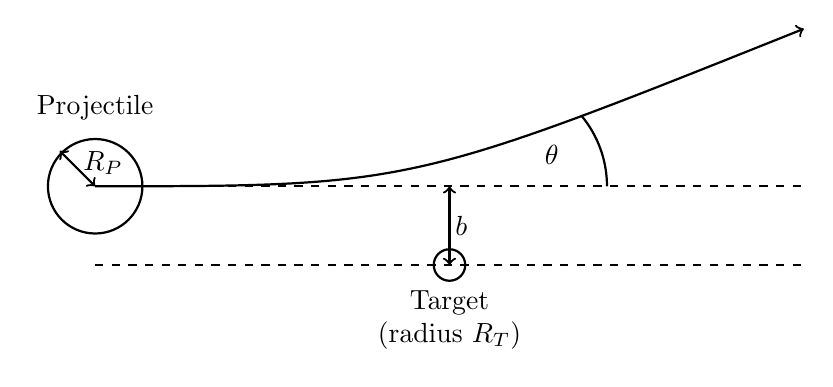
\begin{tikzpicture}
%    \draw[orange,thin] (0.0,0.0) grid (16.0,9.0);

    \draw[->,thick] (2,2) .. controls (6.0,2) .. (11,4);

%    \node [rotate=0,align=left]  at (10,2.7)    {Projected \\ trajectory};
    \draw[dashed,thick] (2,2) -- (11,2);


    \draw[black,thick] (2,2) circle (0.6);
        \draw[<->,thick] (2,2) -- (1.55,2.45);
    \node [rotate=0]  at (2.1,2.3)    {$R_P$};
    \node [rotate=0]  at (2.0,3.0)    {Projectile};
    \draw[<->,thick] (6.5,1) -- (6.5,2);

    % target
    \draw[black,thick] (6.5,1) circle (0.2);
    \draw[black,dashed,thick] (2,1) -- (11,1);
    \node [rotate=0,align=center]  at (6.5,0.3)    {Target \\ (radius $R_T$)};
   \node [rotate=0]  at (6.65,1.5)    {$b$};

   % angle
    \draw[black,thick] (8.5,2) arc (0:40:1.4);
    % \draw[black,dashed,thick] (11,4) -- (11,1);
   \node [rotate=0]  at (7.8,2.4)    {$\theta$};


  \end{tikzpicture}
  \caption{Schematic illustration of the impact parameter.}
  \label{pic:impact}
\end{figure}



\subsubsection{Multiple Coulomb Scattering}

Coulomb scattering occurs when the projectile is deviated from its trajectory due to the interaction with the Coulomb field of the atomic nuclei of the material traversed~\cite{Beringer:1900zz}. 

The particle can be repeatedly subject to small angular Coulomb scattering and so accumulate an angular deviation significantly larger than from the individual interactions. This process, referred to as Multiple Coulomb Scattering (MCS), leads to a wide distribution of scattering angles. It can be quantified by the RMS scattering angle $\langle \Delta x'_\text{MCS} \rangle$ which is well-described the Moli\`{e}re formula~\cite{Beringer:1900zz}
\begin{align}
\langle \Delta x'_\text{MCS} \rangle = \frac{13.6\,\text{MeV}}{\beta \, c \, P} \, Z \, \sqrt{\frac{d}{X_0}} \, \left[ 1 + 0.038 \, \ln \left( \frac{d}{X_0} \right) \right] \, ,
\end{align}
where $d$ is the distance the particle traversed inside the material and $X_0$ is the radiation length that is a characteristic quantity for the target material. 

The radiation length is accessible via tabulated data or by means of the approximated formula depending on the charge $Z_m$, nucleon number $A_m$ and density $\rho_m$ of the target material~\cite{Beringer:1900zz}
%
\begin{align}
  X_0 = \frac{716.4 \, \text{g} \, \text{cm}^{-2} \, A_m}{\rho_m \, Z_m (Z_m+1) \, \ln (287/\sqrt{Z_m})} \, .
\end{align}
%
The radiation length for the most important collimator materials is given in \tabref{tab:radiation_lengths}.

\begin{table}[b]
\centering
\caption{Nuclear charge number $Z_m$, average nuclear mass number $A_m$, density $\rho_m$ and radiation length $X_0$ for different materials. Data taken from~\cite{IPAC15:TUPTY029}.}
\label{tab:radiation_lengths}
\begin{tabular}{lllll}
\toprule
Material & $Z_m$ & $A_m$  & $\rho_m$ {[}g/cm$^3${]} & $X_0$ {[}cm{]}  \\ \midrule
C (CFC)  & 6     & 12.01  & 1.67                    & 25.57          \\
Cu       & 29    & 63.55  & 8.96                    & 1.435          \\
W        & 74    & 183.85 & 19.30                    & 0.35           \\
Mo$_2$C  & 30    & 67.978 & 8.40                     & 1.222         \\ \bottomrule
\end{tabular}
\end{table}

% DATA FROM ELENA FOR FAST IMPLEMENTATION IF NECESSARY
%       element Z       A       rho   X0[g/cm2] X0[cm] 
% 1	Be	4	9.01	1.848	65.19	35.276
% 2	Al	13	26.98	2.7	24.01	8.893
% 3	Cu	29	63.55	8.96	12.86	1.435
% 4	W	74	183.85	19.3	6.76	0.350
% 5	Pb	82	207.19	11.35	6.37	0.561
% 6	C (CFC)	6	12.01	1.67	-	25.57
% 7	C2	6	12.01	4.52	-	9.40
% -	graphite	6	12.01	2.25	42.700	18.978
% -	diamond	6	12.01	3.14	42.700	13.599
% -	B	5	10.8	2.37	52.690	22.232
% -	Ni	28	58.69	8.9	12.680	1.425
% 	O	8	16	-	34.240	-
% -	Al2O3	10	20.392	3.97	27.940	7.038
% 10	Mo	42	95.962	10.22	9.8	0.9589041096
% -	Mo2C	30	67.978	8.4	10.266	1.222
% 8	MoGr	6.653	13.532	2.5	29.828	11.931
% 9	CuCD	11.898	25.238	5.4	17.073	3.162
% 11	Glidcop	28.823	63.149	8.93	12.881	1.442
% 12	Inermet	67.657	166.677	18	6.922	0.385


\subsubsection{Energy Loss from Ionization} 

  \begin{figure}[t]
  \centering
  \includegraphics[width=0.85\textwidth]{pictures/15091401.png}
  \caption{Stopping power as described by the Bethe-Bloch formula~\cite{Beringer:1900zz}. }  
  \label{pic:15091401}
  %/home/phermes/Desktop/lec1.png
  \end{figure}

Particles at the passage through matter can interact inelastically with the electrons of the atoms constituting the target material. At such encounters, a fraction of the projectile's kinetic energy is disposed into the energy required to deliberate an electron from an atom of the target material.

\newpage
Quantitatively, the mean energy loss per traversed length unit (or stopping power) in the material is described by the Bethe-Bloch formula~\cite{Beringer:1900zz}:
\begin{align}
- \frac{1}{\rho_m} \, \left\langle\frac{dE}{dx}\right\rangle = \frac{4 \pi}{\rho \, m_e c^2} \, \frac{nq^2}{\beta^2} \, \left(\frac{e}{4\pi\varepsilon_0}\right)^2 \, \left[\ln \left(\frac{2 \, m_e c^2 \, \beta^2}{I \, (1-\beta^2)}\right) - \beta^2\right] \, , \label{eq:bethe}
\end{align}
where $I$ is the mean excitation energy (which is tabulated for different materials), $m_e$ is the electron rest mass, $q$ is the particle charge, $\rho_m$ is the density of the traversed material and $n$ is the electron density in the material. The stopping power is shown as a function of $\beta \gamma$ of the particle in \figref{pic:15091401}. It increases quadratically with the particle charge. Energy loss from ionization is therefore more important for \lead ions than for protons (see \tabref{tab:physics_ions_matter}).

\subsubsection{Electromagnetic Interactions} \label{chap:emd}
\textit{Electromagnetic Dissociation in Collimators} \newline
Electromagnetic dissociation (EMD) is a photo-nuclear reaction that occurs at ultraperipherical collisions of the involved nuclei \mbox{($b>R_P + R_T$)}. The Lorentz contracted electric fields lead to the exchange of a large number of virtual photons which can induce the nuclear excitation of one or both of the involved nuclei~\cite{PhysRevSTAB17021006}. The cross section of the EMD process scales logaritmically with the relativistic $\gamma$ factor of the impacting nucleus~\cite{PhysRevSTAB17021006}. 

The excited nuclei dissipate the energy acquired under the emission of one or more nucleons, where the emission of neutrons has the largest cross section for heavy nuclei. The process of neutron (n) emission of $m-$th order, triggered by EMD from the interaction with the carbon of the LHC collimators, is summarized by the following reaction formula:
%
\begin{align}
\text{EMD}m: \quad ^{208}\text{Pb}^{82+} &+ ^{12}\text{C} \rightarrow ^{(208-m)}\text{Pb}^{82+}  + ^{12}\text{C} + m \, \text{n} \, .
\end{align}
%
Also higher order EMD processes with the emission neutrons and protons are possible, but have a lower cross section. Overall, the EMD process is very important to consider in the picture of heavy-ion collimation, because the residual ions have rigidities very close to the main beam. As it is demonstrated in \chapref{chap:ir2loss}, they can travel through the magnetic lattice of the LHC over large distances and may cause distinct losses at given LHC elements. The cross-section for photo-nuclear reactions scales proportionally with $Z^2$~\cite{PhysRevSTAB17021006}.

\mbox{} \\
\textit{Electromagnetic Dissociation in Interaction Points} \newline
EMD can also occur from the interaction of colliding particles at the IP. The reaction chain for neutron emission of $m-$th order is the following:
%
%
\begin{align}
   \text{EMD}m:  \quad ^{208}\text{Pb}^{82+} + ^{208}\text{Pb}^{82+} \rightarrow ^{208}\text{Pb}^{82+} + ^{208-m}\text{Pb}^{82+} + m \, \text{n}
\end{align}
%
Again, higher order processes are possible, but the emission of a single neutron has the largest cross section. For example, the emission of one neutron and one proton is suppressed by two orders of magnitude compared to the single neutron emission~\cite{Pshenichnov:prinvate}.
%
\newline \mbox{} \newline
\textit{Bound-Free Pair Production} \newline
The photon exchanged in ultra-peripheral collisions of two ions can create a virtual pair of leptons from which the negatively charged particle may be captured by one of the interacting nuclei. This process is referred to as bound-free pair production (BFPP). Of practical relevance in terms of cross-section are BFPP processes in which electrons are captured. The BFPP process of $m$-th order for LHC \lead ions is summarized as follows~\cite{BFPP1}:
%
\begin{align}
  \text{BFPP}m:  \quad ^{208}\text{Pb}^{82+} + ^{208}\text{Pb}^{82+} \rightarrow ^{208}\text{Pb}^{82+} + ^{208}\text{Pb}^{(82-m)+} + m \, e^+
\end{align}
%%
The cross-section for the first order BFPP processes in which one ion captures an electron can be approximated by the formula:
%
\begin{align}
  \sigma_\text{BFPP} = Z_P^5 \, Z_T^2 \, a \log \left( \frac{\gamma_\text{cm}}{\gamma_0} \right) \, ,
\end{align}
%
where $Z_P$ and $Z_T$ are the charge numbers of the projectile and target, $\gamma_\text{cm}$ is the relativistic Lorentz factor in the center of mass frame and $a,\gamma_0$ are tabulated values with a small dependence on $Z_T$~\cite{PhysRev:63:Meier}. This equation also shows that, compared to processes at the IP, the BFPP cross section for interactions at the collimators is significantly smaller because of the quadratic dependence on $Z_T$ and the reduced $\gamma_\text{cm}$ for a fixed target interaction.
\vspace{0.2cm}

%
Compared to the fully stripped nucleus, the $^{208}\text{Pb}^{(82-m)+}$ ion has a different mass to charge ratio and is therefore subject to dispersion. Already the secondary beam generated from first order BFPP (the dominating process in \lead - \lead collisions at $7\,Z\,$TeV) is outside the momentum acceptance of the LHC arcs and hence lost in the DS magnets at the end of the IR in which it is produced~\cite{PRSTAB:12:071002}. The cross sections for the most important electromagnetic interactions of \lead ions colliding at the IP at $7\,Z\,$TeV are summarized together with the $\chi$ factor quantifying their mass to charge ratio in \tabref{tab:BFPP_cross_section}. 
\vspace{0.2cm}


\begin{table}[t]
\centering
\caption{Cross sections and relative mass to charge ratio of interaction products for electromagnetic and photo-nuclear interactions of colliding \lead beams at 7$\,Z\,$TeV~\cite{schaum:thesis}.}
\label{tab:BFPP_cross_section}
\begin{tabular}{cc ccccc}
\toprule
 & Unit & BFPP1 & BFPP2 & EMD1 & EMD2 & $\sum$ EMD  \\ \midrule
$\sigma$ &  [b] & 281 & 0.006 & 96  & 29 & 226 \\ 
$\chi-1$ & $[10^{-3}]  $  & -12.2  & -24.4  & 4.84  & 9.72  & - \\ 
\multicolumn{1}{c}{Reference}  &       & \cite{PhysRev:63:Meier}  & \cite{EurPhys:74:Artemyev}  & \cite{PRSTAB:12:071002} & \cite{PRSTAB:12:071002} & \cite{PRSTAB:12:071002}       \\ 
\bottomrule
\end{tabular}
\end{table}

%
With the presented cross section and considering the design luminosity, the secondary BFPP1 beam carries a power of 26~W. With its distinct rigidity change, the secondary BFPP beam impacts the DS magnets in a very localized manner. This leads to a locally high power density in the magnet coils that may cause a quench, which was demonstrated in a dedicated BFPP quench test~\cite{accnote_bfpp_quench}. In 2015, dedicated orbit bumps were used in IR1 and IR5 to steer the secondary BFPP beam into an empty cryostat where the lost particles cannot cause a magnet quench. In the region around the ALICE experiment this solution is not applicable, such that for future operation in HL-LHC, the installation of additional collimators in the IR2 DS magnets is envisaged~\cite{IPAC15:TUPTY028}. 


%

%\reference{http://journals.aps.org/pra/pdf/10.1103/PhysRevA.63.032713}

\newpage

\subsubsection{Nuclear Interactions}
\textit{Nuclear Interactions in Collimators} \newline
%
Nuclear encounters with impact parameters smaller or equal to the sum of the radii of the involved nuclei can lead to interactions over strong force. The gluon exchange implies large momentum transfers which may lead to the production of new particles or nuclear fragmentation subsequent to the nuclear excitation of one or both nuclei.

A very important nuclear process for protons interacting with the collimator material is single diffractive scattering. In this process, the proton interacts with a nucleus of the collimator material and is excited to a higher nuclear state. This excited state decays back into a proton and other particles. The momentum of the outgoing proton is reduced with respect to the proton which was initially entering the reaction~\cite{IPAC14:MOPRI077}.


\begin{table}[b]
\caption{Cross sections for EMD1 (single neutron emission) and nuclear interactions of \lead ions for different fixed target materials at the 2011 LHC energy of $3.5\,Z\,$TeV and its design energy $7.0\,Z\,$TeV~\cite{PhysRevSTAB17021006}.}
\label{tab:xsections}
\centering
\begin{tabular}{ccccc}
  \toprule
       & \multicolumn{2}{c}{\begin{tabular}[c]{@{}c@{}}$\sigma$ {[}b{]}\\ $3.5\,Z\,$TeV\end{tabular}} & \multicolumn{2}{c}{\begin{tabular}[c]{@{}c@{}}$\sigma$ {[}b{]} \\ $7.0\,Z\,$TeV\end{tabular}} \\ \midrule
Target & EMD1                                            & Nuclear                                         & EMD1                                            & Nuclear                                         \\ \midrule
C      & 0.471                                          & 3.24                                            & 0.498                                          & 3.26                                            \\
Cu     & 10.16                                          & 5.09                                            & 11.05                                          & 5.11                                            \\
W      & 63.52                                          & 6.92                                            & 68.91                                          & 6.95   \\ \bottomrule                                         
\end{tabular}
\end{table}

For heavy ions, the nuclear excitation of either the target and/or the projectile and their subsequent disintegration leads to a spectrum of residual nuclei much wider than that of EMD processes~\cite{bartke:relativistic}. Typically residual ion fragments from nuclear interactions can cover the full isotope spectrum (with $A<A_0$) and therefore produce particles with rigidities far from the main beam. For the materials used in primary LHC collimators nuclear interactions occur with cross sections almost one order of magnitude above that of EMD1 (see \tabref{tab:xsections}). The mechanism of nuclear fragmentation of \lead ions in the TCP collimator material is summarized by the following reaction formula:
%
\begin{align}
  ^{208}\text{Pb}^{82+} + ^{12}\text{C} \rightarrow ^{A_X}\text{X}^{Z_X+} + ^{A_Y}\text{Y}^{Z_Y+} + ^{12}\text{C} + N_n \, \text{n} + N_p \, \text{p} + ...
\end{align}
Here, $A_X, A_Y$ are the nuclear mass numbers of the fragment $X$ and $Y$, $Z_X,Z_Y$ are their charge numbers and $N_n,N_p$ are the number of produced neutrons and protons. 


Processes of fragmentation, either from EMD or nuclear interactions, cause also deviations in angle and transfer of transverse and longitudinal momentum. The created fragments hence populate not only a wide spectrum in terms of mass and charge, but also in terms of angle (which can dominate over angular scattering from MCS) and momentum. The latter leads to an additional smearing of the distribution of magnetic rigidities and hence loss locations~\cite{PhysRevSTAB17021006}.


\textit{Nuclear Interactions at the IP} \newline
Nuclear fragmentation processes at the IP are the main interest of the LHC experiments. At a momentum of 7$\,Z\,$TeV, the total cross section for such hadronic interactions of two \lead ions is 8\,b~\cite{ALICE:TechnicalProposal}. In terms of quench risk, debris from nuclear fragmentation of \lead ions at the IP is a negligible process compared to the secondary BFPP beam, because the cross section is significantly smaller and the broad spectrum of generated $\chi$-values leads to a wider spread of loss locations. 

For proton operation at high luminosity, physics debris from nuclear interactions can lead to significant loss rates at magnets close to the IP, which motivated the installation of the TCL collimators, because the superconducting Q5 in IR1 or IR5 could quench otherwise.
 

\subsubsection{Nuclear Evaporation and Statistical Fragmentation}

The residual heavy ions generated at a cascade of interactions of either nature may still be in a nuclear charge state above the ground level. Depending on the mass of the fragment, two physical processes of energy dissipation can be distinguished. 

Heavy nuclei can decay into their ground state by either nuclear fission, the emission of nucleons or $\gamma$ rays, a process referred to as nuclear evaporation~\cite{HEP2003:MOMT005}. Proton emission from nuclear evaporation is suppressed compared to neutron emission because of the Coulomb barrier~\cite{HEP2003:MOMT005}.

Light residual ions are subject to fragmentation which can be statistically described by the Fermi breakup model~\cite{fermi:breakup}. In this model, significant momentum can be transferred to the residual fragments.




\subsubsection{Summary and Conclusions}

Interactions of heavy ions with the collimator material can cause changes in transverse and longitudinal momentum. Furthermore, fragmentation processes produce residual particles with changed mass and charge that have large rigidity offsets with respect to the main beam. A summary of the most important processes for the study of heavy-ion interactions with collimators is given in \tabref{tab:physics_ions_matter}. The mean free path $\lambda$ for nuclear interactions and EMD describes the mean distance a particle traverses in the material before it interacts via the respective reaction channel. 

The comparison to protons clearly shows that the nuclear interaction length $\lambda_\text{nuclear}$ for \lead ions is smaller by more than one order of magnitude compared to protons. In addition, the EMD process generates off-rigidity ion fragments. 

\begin{table}[t]
\caption{Characteristic quantities for the most important physical processes of protons and lead ions traversing CFC at 7$\,Z\,$TeV. Data taken from \cite{ICOSIMref02} and scaled to the density of CFC.}
\begin{center}
\begin{tabular}{ c c c c }
\toprule
Physics Process & Unit & Proton & \lead \\ \midrule
$- \frac{dE}{E\,\mathrm{d}x}$ & [$10^{-5}$\,m$^{-1}$] & 11 & 917 \\ 
$\langle \Delta x'_\text{MCS} \rangle$ &  [$\,\mu$rad/$\sqrt{m}$] & 4.0 & 4.0 \\ 
$\lambda_\text{nuclear}$ & [cm] & 47.9 & 3.1 \\ 
$\lambda_\text{EMD}$ & [cm] & - & 23.9 \\ \bottomrule
\end{tabular}
\end{center}
\label{tab:physics_ions_matter}
\end{table}




\subsection{Collimation Cleaning Inefficiency}

Particles which are not absorbed by the TCPs, but instead out-scattered, should be captured by the TCSG collimators. This requires that they receive a sufficient transverse angular kick $\Delta x'$ at the TCP, which is mathematically expressed by the following inequality~\cite{ICOSIMref02}
%
\begin{align}
  \Delta x' > \sqrt{\frac{(N_S^2 - N_P^2) \, \epsilon_N }{ \gamma \, \beta_x } } \,. \label{dx:secon}
\end{align}
%
Here, $\beta_x$ is the horizontal betatron function at the TCP and $N_P$ and $N_S$ are the applied half gaps of the TCP and TCSG respectively. The formula assumes an ideal betatron phase advance between TCP and TCS, such that the particle amplitude at the secondary collimator is maximized. Particles which do not obey the condition defined in \eqref{dx:secon}, may leave the collimation system and continue moving in the machine.  

If, in the course of interacting with the collimator material, they have been subject to significant change of rigidity, they can to be outside of the rigidity acceptance and absorbed in the aperture of the superconducting magnets in the dispersion suppressor where the dispersion increases. 

The local loss rate in the machine aperture from collimation debris is measured by means of the local cleaning inefficiency $\eta(s)$, which quantifies the cleaning performance of the collimation system. For proton losses, it is defined as the number of locally lost protons $N_\text{loc}(s)$ in the interval $[s,s+\Delta s]$, normalized by the number of protons lost at the collimators $N_\text{tot}$~\cite{Bruce2014a}:
%
\begin{align}
  \eta_p(s) = \frac{N_\text{loc}(s)}{N_\text{tot} \, \Delta s} \, . \label{eq:eta:prot}
%\frac{n_p(s)}{n_\text{max} \, \Delta s} \, .
\end{align}
%
This definition is valid if the momenta of the impacting particles are similar. As shown in the previous section, the collimation debris of heavy-ion beams is composed of many different isotopes which can have a large spread in momentum. To take into account the different energetic contributions from the individual particles, the cleaning inefficiency of heavy-ion beams is defined in a more generic manner. Instead of counting the number of lost ions, the total amount of locally lost heavy-ion energy $E_\text{loc}$ in the interval $[s,s+\Delta s]$ is related to the  highest amount of energy lost in the LHC collimators $E_\text{max}$:
%
\begin{align}
  \eta(s) = \frac{ E_\text{loc} (s)  }{E_\text{max} \, \Delta s} \, . \label{eq:eta:ions}
\end{align}
%
%
The local cleaning inefficiency allows a simple scaling of the total loss rate to the amount of locally lost energy. Note that the above definition of the cleaning inefficiency considers a particle loss as the point of interception with the aperture of the beam pipe. In measurements of the losses in the LHC, this definition is not applicable, because secondary showers created by the particles interacting with the material at the location of impact are measured. The measurement of beam losses in the LHC is presented in the next section.

% Following the definition of $\eta(s)$ and \eqref{eq:taudef}, the power $P_L(s,t)$ deposited at the location $s$ with the local cleaning inefficiency $\eta(s)$ is given by
% %
% %
% \begin{align}
%   P_L(s,t) = \eta(s) \, \frac{N(t)}{\tau} = \eta(s) \, P_\text{TCP} \, ,
% \end{align}
% %
% where $P_\text{TCP}$ is the power load on the primary collimator.

% The high production rate of off-rigidity particles with heavy-ion beams is the origin of the worse cleaning inefficiency compared to proton beams. A dedicated simulation to understand the effect in more detail is presented in \chapref{colleff:ions}.

\subsection{Measurement of Losses in LHC Operation} \label{chap:lossmeas}
%
\begin{figure}[htbp]  
    \centering
    \includegraphics[width=0.8\textwidth]{pictures/16033101.pdf}
    \caption{Top: Ionization chambers of the LHC BLM system, mounted at the LHC Magnets. Bottom: Inner structure of an ionization chamber. Figures taken from \cite{BLM_homepage}.}  
    \label{pic:16033101}
    %/home/phermes/Desktop/pictures/pic.pdf
\end{figure}

The LHC is equipped with more than 4500 ionization chambers, the beam loss monitors (BLM)~\cite{BLMref1,BLMref02}, with the aim of keeping track of the particle losses throughout the ring. They are installed at the outer side of superconducting magnets, collimators and other locations. The ionization chambers are gas filled cylinders housing a structure of parallel electrodes operated with opposite voltages (see Fig.~\ref{pic:16033101}). Charged particles traversing the detector ionize the gas particles and the created ions and their electrons are captured by the electrodes, which is measured as a drop of the high voltage at which the BLMs are operated. The measured signal is proportional to the radiation dose.
%



%\input{pictures/16070406.tex}
  % #PHTHESIS FILE ORIGIN
  %/home/phermes/Dropbox/PhD/pictures/160704_blms/drawing.tex
%


\begin{figure}[htbp]
  \centering
  \begin{tikzpicture}
    \node[anchor=south west,inner sep=0] (image) at (0,0) {\includegraphics[width=1.0\linewidth]{pictures/16072802.pdf}};

  % \draw[help lines,step=.2] (0,0) grid (16.0,9.0);
  % \draw[help lines,line width=.6pt,step=1] (0,0) grid (16.0,9.0);
  % \foreach \x in {0,1,2,3,4,5,6,7,8,9,10,11,12,13,14,15,16}
  %      \node[anchor=north] at (\x,-0.1) {\x};
  % \foreach \y in {0,1,2,3,4,5,6,7,8,9}
  %     \node[anchor=east] at (-0.2,\y) {\y};

    \node [x={(image.south east)},y={(image.north west)}]                   at (0.07,0.50)    {MB};
    \node [x={(image.south east)},y={(image.north west)}]                   at (0.23,0.50)    {MQ};
    \node [x={(image.south east)},y={(image.north west)}]                   at (0.48,0.50)    {MB};
    \node [x={(image.south east)},y={(image.north west)}]                   at (0.83,0.50)    {MB};
    
    %\node [draw,rotate=0 ,x={(image.south east)},y={(image.north west)}]                   at (0.22,0.96)    {text1};
    %\node [draw,rotate=0 ,x={(image.south east)},y={(image.north west)},anchor=west]       at (0.22,0.80)    {text2};
    %\draw[->,color=black,thick,x={(image.south east)},y={(image.north west)}]             (0.42,0.22) -- (0.37,0.23);
  \end{tikzpicture}
  \caption{BLM positioning around a MQ magnet~\cite{lechner:blmpos}. }  
  \label{pic:16071902}
  %/home/phermes/Desktop/drawing.pdf
  \end{figure}




The BLMs measure the secondary particle showers from the interaction of beam particles with the material of collimators or with the beam pipes and surrounding components. Given their small size, the positioning of the BLMs is essential to monitor the loss rate at strategic locations where high losses are expected. A schematic illustration of the BLM positioning around the superconducting magnets in the LHC arcs is shown in \figref{pic:16071902}. 


\newpage


\begin{table}[b]
\centering
\caption{Summary of LHC BLM integration times~\cite{DIPAC05:POW019}.}
\label{tab:RS}
\small
\begin{tabular}{cc} \toprule
Running Sum & Integration Time (ms) \\ \midrule
1           & 0.04                  \\
2           & 0.08                  \\
3           & 0.32                  \\
4           & 0.64                  \\
5           & 2.56                  \\
6           & 10.24                 \\
7           & 81.92                 \\
8           & 655.36                \\
9           & 1310.72               \\
10          & 5242.88               \\
11          & 20971.52              \\ \bottomrule
\end{tabular}
\end{table}

The BLM data is continuously monitored by the LHC interlock system which triggers a beam dump if defined thresholds are exceeded~\cite{guaglio2005reliability}. Both the quench limit and the intensity limit at which the physical integrity of the collimators is endangered by beam induced plastic deformations, depend on the time scale at which the losses occur~\cite{bertarelli:chamonix11,BIQ14:Redaelli}. Therefore the signals of the ionization chambers are sampled over twelve different integration time scales reaching from 40\,$\mu$s to $83.89\,$s. The different integration times are denominated running sums (RS) and reach from RS01 to RS12 (see \tabref{tab:RS}). With increasing RS, the BLM thresholds are set to larger values, accounting for the larger quench limit with increasing loss duration. 

It is not straight-forward to deduce the number of locally lost particles and the energy deposition in the magnet coils from measured BLM signals. One reason for this is the limited azimuthal and longitudinal coverage of the BLMs. Furthermore, at every location and for every beam loss scenario, a different response function relates the measured signal to upstream particle impacts at the beam pipe. Therefore, the BLM signals should be interpreted on a global scale to identify critical loss locations in the machine, rather than deducing quantitative information about energy deposition. The latter requires dedicated simulations, including the shower propagation from the point of primary particle impact~\cite{PAC09:TH5RFP035,Bruce2014a,PhysRevSTAB.18.061002}. Such shower propagation simulations can be combined with quench limit estimates to derive operational thresholds for the BLMs.

The longitudinal distribution of losses in the LHC ring is referred to as a loss map. The constant loss monitoring in operation (physics loss map) delivers a convolution of all losses presently occurring, whatever their origin might be. The qualification of the LHC collimation system is carried out in dedicated measurements, presented in detail in \chapref{chap:qualification_lossmaps}.
%



\chapter{Simulation Tools} \label{chap:simtools}

Important contributions to the excellent performance of the LHC came from theoretical simulations. Many tools have been developed and used to predict various physics aspects of the machine. For collimation, particularly software for particle tracking and simulations of particle-matter interaction are important. The former requires also a detailed model for optics computation, since the configuration of the magnetic lattice is crucial for the particle motion in the machine. In order to have a complete picture of the collimation efficiency, information must be exchanged between the tracking tool and the particle-matter interaction, which can be realized in different manners. In this chapter, different software tools which are important for the development of an improved heavy-ion collimation simulation tool are presented.



\section{MAD-X}
MAD-X (Methodical Accelerator Design)~\cite{MADXref01} is the standard tool at CERN to simulate beam dynamics and compute beam optics in particle accelerators. The software is a complete migration of MAD-8 (written in FORTRAN77) to C++ and was introduced in 2002 for the design and simulation of the LHC optics~\cite{MADXref02}.

The structure of the machine and the strengths of the magnets are given by the user by means of dedicated input files. A matching function provides the functionality to adjust specific variables such that  defined constraints are fulfilled. An aperture model of the machine can be processed and compared with the beam position and dimensions to evaluate the available normalized aperture throughout the machine. A dedicated function produces the required optics input for SixTrack (see below). 



% ----------------------------------- PARTICLE MATTER INTERACTION ----------------------------------

\section{FLUKA}


\begin{figure}[t]  
    \centering
    \includegraphics[width=0.8\textwidth]{pictures/16060102.pdf}
    \caption{FLUKA geometry of the three primary collimators in IR7 for B1~\cite{skordis_fluka_model}.}  
    \label{pic:16031201}
    %/home/phermes/Dropbox/PhD/pictures/160601_fluka_collimators/annotated/coooo_annotated.pdf
\end{figure}


FLUKA (FLuktuierende KAskade) is a fully integrated Monte-Carlo package to simulate particle transport and the interaction of particles with matter~\cite{ferrari2005fluka,bohlen2014fluka}. The package simulates the interaction of a primary beam particle with the nuclei of the traversed material in a user-defined 3D geometry. It also simulates the particle-matter interaction of particles generated in electromagnetic or hadronic cascades. The software uses regularly updated physics models derived from experimental data and is used for a variety of applications, including particle shower simulations and energy deposition studies in the LHC. 

The species, energy and direction of the incident particles are given by the user in a dedicated input file. The geometry can be defined manually with a dedicated syntax or generated from the FLUKA element database (fedb) which contains LHC elements which may be assembled~\cite{WEPPD071}. The full geometry of the different LHC IRs is available as a FLUKA model and is regularly used to study energy deposition, activation or shower propagation for different beam loss scenarios. As an example, the geometry of three primary LHC collimators, including their supports, is shown in \figref{pic:16031201}.

The FLUKA user input file is a sequence of command lines (called \textit{cards}), which define the simulation setup via different available options. The required output information can be selected, post-processed and written to dedicated files via 38 different user routines that can be linked to the FLUKA executable. Each user routine consists of FORTRAN code that can be adjusted to the specific requirements of the user. The options for a pre-defined output can be set in the FLUKA input file by means of the respective card linked to the specific user routine. 


\section{SixTrack}

\subsection{Tracking in SixTrack}

SixTrack~\cite{SixTrackref01,SixTrackref03,SixTrackref02,SixTrackref04} is designed to provide symplectic (see \chapref{chap:hamiltonian}) six-dimensional tracking of relativistic proton beams in high-energy synchrotrons over many turns. Initially developed for dynamic aperture studies, the software is subject to regular updates providing new features for dedicated functions or improved physics models. The tracking algorithm is based on symplectic tracking maps derived from the accelerator Hamiltonian. Tracking maps are transformation rules for the six-dimensional particle coordinates describing the effect of the beam line element on the particle. Based on these tracking maps, the six-dimensional particle coordinates are transported element by element through the magnetic lattice of the accelerator. The symplecticity (see \chapref{chap:hamiltonian}) makes SixTrack an excellent tool to provide accurate tracking over a large number of turns. The tracking is performed around the reference orbit which is known from the optics computation. 



\subsection{Collimation SixTrack}



SixTrack is equipped with a collimation subroutine~\cite{1591725,collsixtrack} providing an integrated environment for 6D thin-lens tracking together with a Monte-Carlo module to simulate the interaction of the protons with the material of the collimation devices. For this purpose, physics models and cross-sections for different types of interactions are implemented for different collimator materials. The SixTrack particle-matter interaction simulation includes energy loss via ionization, multiple Coulomb scattering and nuclear interactions at the passage of the protons through the collimator. Both elastic and inelastic nuclear interactions are simulated, where the proton is considered to be lost when the interaction is inelastic, except in the case of single diffractive scattering. For particles having undergone single diffractive and elastic scattering, the tracking is continued when the particle has left the collimator.


In order to identify the loss distribution in the ring, the individual particle tracks are compared to a detailed model of the LHC aperture. The aperture check is first carried out at dedicated aperture markers to reduce the required computing time. Beginning from the marker, particle track is then reversely extrapolated as a straight line and the aperture check is iteratively repeated in steps of $10\,$cm until the loss location is identified.  In the current SixTrack release version\footnote{SixTrack Version 4.5.34 from 20.04.2016.}, this algorithm is executed on a post-processing level by means of the software \texttt{BeamLossPattern}~\cite{ChamonixXIV:BLP} (see \figref{pic:15070701}). Given that all particle tracks have to be saved and analyzed in this approach, this method of loss detection is very time- and space-consuming. 






An important recent extension of SixTrack is an online aperture check during the tracking, instead of computing the aperture losses on a post-processing level. With this algorithm, SixTrack continuously compares the particle coordinates to a detailed model of the LHC aperture while tracking. With the initial aperture check carried out at the markers, the losses are precisely localized by backwards extrapolation, equivalent to the aperture check with \texttt{BeamLossPattern}. The approach significantly reduces the required CPU time and the amount of  generated data.


\begin{figure}[htbp]
  \centering
  \begin{tikzpicture}
    \footnotesize
    \node[anchor=south west,inner sep=0] (image) at (0,0) {\includegraphics[width=0.50\linewidth]{pictures/16080201.pdf}};
    \node [x={(image.south east)},y={(image.north west)}]                   at (0.79,0.40)    {$\Delta s = 10\,$cm};
    \node [x={(image.south east)},y={(image.north west)}]                   at (0.5,-0.050)    {Position [km]};
    \node [rotate=90,x={(image.south east)},y={(image.north west)}]                   at (-0.05,0.5)    {$x$ [mm]};
    \node [x={(image.south east)},y={(image.north west)}]                   at (0.2,0.9)    {Aperture};
    %\node [draw,rotate=0 ,x={(image.south east)},y={(image.north west)}]            a       at (0.22,0.96)    {text1};
    %\node [draw,rotate=0 ,x={(image.south east)},y={(image.north west)},anchor=west]       at (0.22,0.80)    {text2};
    %\draw[->,color=black,thick,x={(image.south east)},y={(image.north west)}]             (0.42,0.22) -- (0.37,0.23);
  \end{tikzpicture}
  \caption{Illustration of the \texttt{BeamLossPattern} algorithm to identify aperture losses from particle tracks simulated with SixTrack. Figure taken from~\cite{ChamonixXIV:BLP}.}  
  \label{pic:15070701}
  %/home/phermes/backtrack/drawing-compiled.pdf
  \end{figure}


Options and input for the execution of Collimation SixTrack are given via dedicated input files:
\begin{itemize}
  \item \texttt{fort.2}: Defining the optical configuration of the accelerator. This file can be automatically generated from MAD-X.
  \item \texttt{fort.3}: Selection of options and beam settings via dedicated blocks. The most relevant options for collimation studies are the number of tracked particles, number of turns through the machine, particle energy, RF settings, collimator settings and initial distribution. 
 \item \texttt{CollDB}: Collimator database file, containing information on the name, length and material of the different collimators.
 \item \texttt{allapert}: Contains detailed information about the beam pipe aperture throughout the ring.
\end{itemize}

The \texttt{COLLIMATION} block in the \texttt{fort.3} file contains information about the settings of the different collimator families. Collimator families are classified by the prefix of the collimator name and the region where the collimator is installed. 




The initial particle distribution can be selected from different options. In the framework of this document, two of them are of major importance: the annular halo and the direct halo~\cite{Bruce2014a}, as shown in \figref{pic:16080202}. The annular halo is a hollow ellipse in the horizontal or vertical phase space with a normalized amplitude between $N_P$ and $N_P+\bar{\epsilon}$, where $N_P$ is the normalized half gap of the primary collimator and $\bar{\epsilon}$ is a small quantity. The quantity $\bar{\epsilon}$ accounts for the diffusion which is not taken into account in SixTrack, in order to save computing time~\cite{Bruce2014a}. The annular halo is typically sampled at IP1, with a Gaussian distribution in the other plane. 

The particles hit the primary collimator within several turns, depending on their initial betatron phase. The selection of an appropriate value for $\bar{\epsilon}$ requires to assume the impact parameter at the collimator jaw (the transverse distance of the impacting particle from the edge of the collimator jaw, see \figref{pic:impactpar}). It is, however, altered by non-linearities in the machine from higher order fields than quadrupoles, which deform and shift the phase space ellipse~\cite{Bruce2014a}. This effect is discussed in more detail in \chapref{chap:pha_shift}. The direct halo is simulated to impact immediately at the TCP jaws, which allows for a direct control of the impact parameter and reduces the number of turns required for the tracking.


\begin{figure}[t]  
  \centering
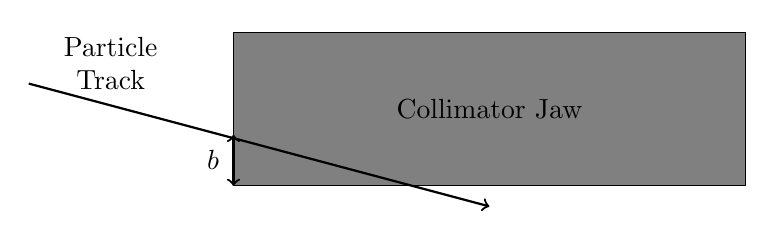
\begin{tikzpicture}[scale=1.3]
  % helper grid: comment for final drawing
  % \draw[help lines,step=.2] (0,0) grid (16.0,9.0);
  % \draw[help lines,line width=.6pt,step=1] (0,0) grid (16.0,9.0);
  % \foreach \x in {0,1,2,3,4,5,6,7,8,9,10,11,12,13,14,15,16}
  %      \node[anchor=north] at (\x,-0.1) {\x};
  % \foreach \y in {0,1,2,3,4,5,6,7,8,9}
  %     \node[anchor=east] at (-0.2,\y) {\y};
  \filldraw[fill=gray, draw=black] (3,2) rectangle (8,3.5);
  \draw[->,thick] (1,3.0) -- (5.5,1.8);
  \draw[<->,thick] (3.0,2.0) -- (3.0,2.5);
  \node[align=center]  at (1.8,3.2)  {Particle\\ Track};
  \node  at (5.5,2.75)  {Collimator Jaw};
  \node  at (2.8,2.25)  {$b$};
\end{tikzpicture}
  \caption{Illustration of the impact parameter $b$.}
  \label{pic:impactpar}
  \end{figure}

Besides these halo types which can be generated by SixTrack, the software is capable of reading an input file containing the 6D coordinates of the particle distribution to be tracked.




\begin{figure}[b]
  \centering
  \begin{tikzpicture}
    \node[anchor=south west,inner sep=0] (image) at (0,0) {\includegraphics[width=0.7\linewidth]{pictures/16080202.png}};
    %\node [draw,rotate=90,x={(image.south east)},y={(image.north west)}]                   at (0.50,0.50)    {text0};
    %\node [draw,rotate=0 ,x={(image.south east)},y={(image.north west)}]                   at (0.22,0.96)    {text1};
    %\node [draw,rotate=0 ,x={(image.south east)},y={(image.north west)},anchor=west]       at (0.22,0.80)    {text2};
    %\draw[->,color=black,thick,x={(image.south east)},y={(image.north west)}]             (0.42,0.22) -- (0.37,0.23);
  \end{tikzpicture}
  \caption{Initial distribution sampled as an annular halo (left panel) and as a direct halo (right panel). Figure courtesy of \cite{Bruce2014a}. }  
  \label{pic:16080202}
  %/home/phermes/Dropbox/PhD/thesis/chapters//home/phermes/Desktop/ann.png
  \end{figure}

 

Collimation simulations with SixTrack are usually carried out for 200 turns with an initial sample of 6.4 million protons to gain enough statistics. In this scenario, one proton lost in the aperture leads to a cleaning inefficiency of $1.5 \times 10^{-6} \, \text{m}^{-1}$ over a 10~cm bin, about one order of magnitude below the estimated quench level during the design of the LHC. Given the large amount of required space which has to be allocated for the aperture loss detection, the simulations are split into 1000 sub-simulations which are submitted to the CERN batch computing service~\cite{cernBatch}. 

In the latter, they are processed in parallel, if possible. The post-processing is carried out on the virtual machine of the cluster, such that only the relevant output is saved back in the user directory and the disk space which has to be allocated  is reduced by several orders of magnitude. 


Additional information can be obtained by a subsequent shower propagation simulation with FLUKA. This allows for the study of energy deposition in the machine hardware, in particular the superconducting magnets, including contributions from hadronic and electromagnetic showers. The input for the subsequent simulation is obtained by SixTrack, which saves the information on particles having undergone inelastic interactions in the collimators to a dedicated file.  Furthermore, the shower simulations can be used to quantitatively predict the resulting BLM signals. Compared to the nominal cleaning simulations with SixTrack these simulations are extensive in terms of time and space consumption and are therefore only carried out for dedicated configurations, e.g. when experimentally measured quench limits shall be theoretically accessed.


\section{SixTrack-FLUKA Coupling}

\begin{figure}[b]  
    \centering
    \includegraphics[width=0.65\textwidth]{pictures/16060101.pdf}
    \caption{Principle of the SixTrack-FLUKA coupling. At every collimator extraction marker (red) the particle bunch is sent to FLUKA where the interaction with the collimator is simulated. The resulting distribution is then re-injected in SixTrack at the injection marker (green), from where the tracking is continued.}  
    \label{pic:16060101}
    %/home/phermes/Dropbox/PhD/pictures/160601_six_fluka_coupling/test/annotated/drawing_annotated.pdf
\end{figure}


The SixTrack-FLUKA active coupling~\cite{mereghetti_ipac2013_1} is a dedicated framework in which the two simulation codes SixTrack and FLUKA are run in parallel to perform beam-machine interaction studies. In particular, the framework is applied to simulate the cleaning performance of the collimation system by complementary tracking in accelerator lattices and particle-matter interaction at the collimators. 

The SixTrack-FLUKA coupling can be used as an alternative to the built-in scattering in SixTrack and instead simulate the beam-matter interaction with FLUKA. It combines the advantages of both codes with their detailed and regularly updated physics models. The backbone of the particle exchange is the use of a network port and a C library to handle TCP/IP network messages. 
This shortens the required simulation time compared to having to reinitialize each code after each particle exchange.


\begin{figure}[t]
  \centering
  \begin{tikzpicture}
    \node[anchor=south west,inner sep=0] (image) at (0,0) {\includegraphics[width=1.0\linewidth]{pictures/16070701.png}};
    %\node [draw,rotate=90,x={(image.south east)},y={(image.north west)}]                   at (0.50,0.50)    {text0};
    %\node [draw,rotate=0 ,x={(image.south east)},y={(image.north west)}]                   at (0.22,0.96)    {text1};
    %\node [draw,rotate=0 ,x={(image.south east)},y={(image.north west)},anchor=west]       at (0.22,0.80)    {text2};
    %\draw[->,color=black,thick,x={(image.south east)},y={(image.north west)}]             (0.42,0.22) -- (0.37,0.23);
  \end{tikzpicture}
  \caption{Collimator models in the FLUKA input file used for the SixTrack-FLUKA coupling.}  
  \label{pic:16070701}
  %/afs/cern.ch/work/p/phermes/private/150629_coupling_ions/hiSix/160315_HLLHC//home/phermes/Desktop/fedb.png
  \end{figure}



The basic principle of the SixTrack-FLUKA coupling is illustrated in \figref{pic:16060101}. The magnetic lattice used in a regular SixTrack simulation is expanded by additional collimator extraction markers at which \mbox{SixTrack} sends the particle distribution to FLUKA, where the interaction with the collimator is simulated. At the end of the collimator, the distribution of residual particles is sent back to SixTrack and re-injected into the lattice at a dedicated injection marker from which the tracking is continued. 

The marker locations correspond to the beginning and end of the collimator tanks. The FEDB stores detailed models of the individual collimator components for each collimator type. The settings for each collimator are loaded in a dedicated pre-processing algorithm and the FLUKA input file is populated with all the necessary collimators based on the FEDB models (see \figref{pic:16070701}). Residual protons which are not identical to the incoming protons (e.g. those produced in nuclear interactions) are assigned to a new particle ID. 

Losses at the aperture of the LHC magnets are identified by the online aperture check. The input for subsequent energy deposition simulations can be obtained in full analogy to that of SixTrack, by saving the positions of inelastic interactions in the collimator jaws.  As an alternative, a \texttt{toucMap} file can be generated, which contains the first collimator impact of each proton at each turn.


\section{ICOSIM}

It was yet anticipated in the LHC design phase that the interaction of the heavy ions with the collimator material can lead to fragmentation into other isotopes, with consequences on the cleaning inefficiency. This was incorporated into a dedicated simulation software for heavy-ion collimation, called Ion Collimation Simulation (ICOSIM)~\cite{ICOSIMref02,ICOSIMref01}. 
\vspace{0.2cm}

It is an integrated program for particle tracking with a Monte-Carlo module to simulate the interaction of heavy ions with the collimator materials. The tracking routine is split in two stages: first, the impact distribution at the TCPs is determined by a linear transformation between them. Every 100 turns, random transverse kicks are applied to the particles to simulate diffusion. When all particles have impacted the TCPs, the tracking of the residual fragments is continued based on a matrix multiplication with chromatic modeling in linear approximation, including sextupole fields in thin-lens approximation. The information about the magnetic lattice is read from MAD-X output. Along with the tracking, the particle amplitudes are compared to a simplified aperture model in which the aperture cross sections are approximated by an ellipse. Once the aperture is identified to be intercepted at the end of an element, the exact location is determined by linear extrapolation, as described in the previous section. 
\vspace{0.2cm}

The Monte-Carlo module simulates the interaction of the ions with matter, including energy loss from ionization via the Bethe-Bloch equation and multiple Coulomb scattering, as well as fragmentation processes from EMD and NF~\cite{ICOSIMref02}. The latter is computed using tabulated cross-section information for the two processes which was generated beforehand with FLUKA or the Pshenichnov model~\cite{ICOSIMref02}. When a particle is subject to fragmentation in the collimator, the heaviest fragment is given back to the tracking routine. Momentum transfers (both transverse and longitudinal) from the fragmentation process are not taken into account~\cite{ICOSIMref02}. At the time of development, these simplifications were considered to be of small importance for the simulation result, because the transverse momentum transfer from the fragmentation process and the energy loss related to it are small compared to the total energy of the ion~\cite{ICOSIMref02}.



\chapter{Collimation of Heavy-Ion Beams} \label{chap:collhi}


The LHC collimation system was designed to efficiently remove the halo of proton beams. While this purpose is well accomplished, the cleaning performance for \lead operation is measured to be significantly worse. In this chapter, the experimental findings on the heavy-ion collimation efficiency are presented and compared to simulations with ICOSIM. Despite limitations that only became apparent after the first feedback from heavy-ion operation, this code provided the state-of-the-art for heavy-ion beam collimation before the LHC was started. It is important to understand in detail its implementation and limitations before embarking for the development of a further improved simulation tool

\section{Qualification Loss Maps}\label{chap:qualification_lossmaps}

The cleaning performance of the LHC collimation system must be validated before it is operated with high intensity beams~\cite{EPAC06:TUPLS018}. This is done by inducing artificial beam losses at the primary collimators and measuring the collimation debris throughout the ring with the LHC BLM system. Qualification loss maps are measured with very low intensity (with a maximum of $3\times 10^{11}$ charges in the machine), compared to  physics operation. The measurements take place when new optics, collimator settings or particle momenta are commissioned. High beam intensities are only allowed to be injected in the LHC if the collimation system was qualified beforehand. 
\vspace{0.2cm}

To induce losses at the IR7 TCP, different strategies to increase the transverse emittance have been developed. Loss map measurements in early LHC operation have been carried out by means of optics changes that led to tune resonance crossing, inducing fast beam losses at the collimation system. Since 2012, the beam excitation is carried out using the transverse damper (\acrshort{ADT})~\cite{Moens:1574590} which can introduce white noise excitation such that the beam particles receive random transverse kicks, resulting in an effective increase of the transverse emittance. The excitation with the ADT is distinguished by the better controllability and can be carried out selectively for both planes of both beams with a selectable loss rate~\cite{Moens:1574590}. Loss maps measured in this approach are referred to as betatron loss maps. The full qualification of the collimation system includes also off-momentum loss maps where the primary losses are induced at the IR3 TCP~\cite{Moens:1574590}. They shall not be further discussed in this work.


% This approach produces loss patterns significantly different from nominal operational losses, in which the losses occur for both planes of both beams, indistinguishable with respect to their origin. In the latter scenario, another loss type could be dominating the global loss pattern and the collimation losses could be too small to be above the background signal of the BLM system. 


% \begin{figure}[htbp]
%   \begin{center}
% \includegraphics[width=0.6\textwidth]{pictures/15102003.pdf}
% \includegraphics[width=0.6\textwidth]{pictures/15091802.pdf}
% \caption{ The upper plots show the full LHC ring, the bottom plots a zoom to IR7.}
% \label{fig:meas_lm_comparison}
%   \end{center}
% \end{figure}


\begin{figure}[htbp]
  \centering
  \begin{tikzpicture}
    \small
    \node[anchor=south west,inner sep=0] (image) at (0,0) {\includegraphics[width=1.0\linewidth]{pictures/16081202.pdf}};
    \node [fill=white,x={(image.south east)},y={(image.north west)}]                   at (0.16,0.92)    {\lead beam};
    \node [fill=white,x={(image.south east)},y={(image.north west)}]                   at (0.16,0.48)    {Proton beam};
    \node [fill=white,x={(image.south east)},y={(image.north west)}]                   at (0.42,0.45)    {Beam};

    \footnotesize
    \node [rotate=90,fill=white,x={(image.south east)},y={(image.north west)},align=center]                   at (0.25,0.29)    {Momentum \\ collimation};
    \node [rotate=90,fill=white,x={(image.south east)},y={(image.north west)},align=center]                   at (0.72,0.29)    {Betatron \\  collimation};

    \node [rotate=90,fill=white,x={(image.south east)},y={(image.north west)},align=center]                   at (0.60,0.29)    {Dump \\  protection};

    %\node [draw,rotate=0 ,x={(image.south east)},y={(image.north west)}]                   at (0.22,0.96)    {text1};
    %\node [draw,rotate=0 ,x={(image.south east)},y={(image.north west)},anchor=west]       at (0.22,0.80)    {text2};
    \draw[->,color=black,x={(image.south east)},y={(image.north west)}]             (0.37,0.42) -- (0.47,0.42);
  \end{tikzpicture}
  \begin{tikzpicture}
    \small
%    \node[anchor=south west,inner sep=0] (image) at (0,0) {\includegraphics[width=1.0\linewidth]{pictures/16081201.pdf}};
    \node[anchor=south west,inner sep=0] (image) at (0,0) {\includegraphics[width=1.0\linewidth]{pictures/16091801.pdf}};

    \node [fill=white,x={(image.south east)},y={(image.north west)}]                   at (0.56,0.46)    {Proton beam};

    \footnotesize
    \node [fill=white,x={(image.south east)},y={(image.north west)}]                   at (0.78,0.890)    {\lead};

    \node [fill=white,x={(image.south east)},y={(image.north west)}]                   at (0.39,0.90)    {DS1};
    \node [fill=white,x={(image.south east)},y={(image.north west)}]                   at (0.435,0.90)    {DS2};
    \node [fill=white,x={(image.south east)},y={(image.north west)}]                   at (0.495,0.90)    {A1};
    \node [fill=white,x={(image.south east)},y={(image.north west)}]                   at (0.64,0.90)    {A2};
    \draw[->,color=black,x={(image.south east)},y={(image.north west)}]             (0.87,0.82) -- (0.84,0.78);
    \node [fill=white,x={(image.south east)},y={(image.north west)}]                   at (0.89,0.84)    {A3};


    %\node [draw,rotate=90,x={(image.south east)},y={(image.north west)}]                   at (0.50,0.50)    {text0};
    %\node [draw,rotate=0 ,x={(image.south east)},y={(image.north west)}]                   at (0.22,0.96)    {text1};
    %\node [draw,rotate=0 ,x={(image.south east)},y={(image.north west)},anchor=west]       at (0.22,0.80)    {text2};
    %\draw[->,color=black,thick,x={(image.south east)},y={(image.north west)}]             (0.42,0.22) -- (0.37,0.23);
  \end{tikzpicture}
  \caption{B1H qualification loss maps measured in 2011 with proton~\cite{Bruce2014a} and \lead beams~\cite{phermes_hb2014} at $3.5\,Z\,$TeV with identical collimator settings and optics, except in IR2. The longitudinal coordinate describes the distance from IP1. The vertical dashed lines mark the LHC octants. The BLM signals are normalized with respect to the highest measured BLM signal. Top: full LHC ring, bottom: zoom to IR7. }  
  \label{fig:meas_lm_comparison}
  %/media/phermes/local/141003_compareICOSIMSixTrackMeasurement/thesis/CompareExperimentalData_LHC_thesis.pdf
  \end{figure}


Loss maps are shown as a mapping of the BLM signals, normalized with respect to the highest measured BLM signal, as a function of the distance from IP1. A color code is applied to distinguish between losses at collimators (black), in normal conducting regions (red) and in the superconducting LHC magnets (blue). 

\mbox{} \\ 
\textit{Heavy-Ion and Proton Qualification Loss Maps measured in 2011} \\ 

The horizontal B1 (B1H) betatron qualification loss maps measured in the 2011 with protons and \lead ions at  $3.5\,Z\,$TeV are directly compared in Fig.~\ref{fig:meas_lm_comparison}. The beam are squeezed in the experimental IRs with the $\beta^*$ values listed in \tabref{tab:betastar}. The optics are identical in the full ring, except in IP2, where the injection settings with $\beta^*=10\,$m are maintained for protons and the heavy-ion beams are squeezed to $\beta^*=1\,$m. The collimator settings are listed in \tabref{tab:14070901}.  

In both qualification loss maps, the collimation regions IR3 and IR7 capture the largest amount of losses. The zoom to IR7 shows not only high losses at the TCP, TCSG and TCLA collimators, but also in the warm magnets in between. These loss signals are mostly induced by shower particles that are generated in the collimators. The magnets in IR7 which are close to the collimators are normal conducting, so these losses do not define a quench risk. 

The measured losses at the TCP in the momentum cleaning insertion IR3 with \lead beams are two orders of magnitude above the signal measured with protons. This can be interpreted as a larger amount of off-rigid particles that is scattered out of the collimators in IR7. While for protons the measured loss signals are beyond the noise level only in regions close to collimators, the loss distribution of heavy-ion beams shows pronounced loss spikes at amplitudes up to $10^{-2}$ in superconducting regions across the LHC ring. 

In both qualification loss maps, the highest loss signal in superconducting magnets is measured in the DS region downstream of IR7 with amplitudes of $3 \times 10^{-4}$ for protons and $2 \times 10^{-2}$ for \lead ions. The losses in the DS have a characteristic structure with two subsequent loss clusters DS1 and DS2 located in the cells 9 and 11. The loss clustering can be explained by the local horizontal dispersion function starting from the TCP, which is also shown in \figref{fig:meas_lm_comparison}.

The loss clusters are located in regions where the local horizontal dispersion function increases, due to the strong fields in the magnetic bending dipoles downstream of IR7. The increasing dispersion guides particles with rigidity offsets into the aperture of the superconducting magnets, where they are lost. Accordingly, the outermost edge of the clusters is located at the quadrupoles in cell 9 and 11, where the dispersion functions have local maxima. Also the loss spikes in the LHC arcs (A1 to A3) that are measured with heavy-ion beams are located at positions where the dispersion function and hence the dispersive offset of off-rigid particles is maximum.

\newpage
The IR7 DS is the superconducting region in the LHC that is exposed to the largest amount of collimation debris. The magnets in this region have the highest risk of beam-induced quenches. The comparison shows that, with heavy ions, the cleaning performance in this region is almost two orders of magnitude worse than for protons. 


\mbox{} \\ 
\textit{Conclusions} \\
While the stored beam energies with heavy-ion beams that were foreseen in the LHC design phase\citedr\, are lower by two orders of magnitude, the collimation losses in the IR7 DS are larger by the same amount. This shows that the quench risk with heavy-ion beams is comparable to that in proton operation. Therefore, the collimation system with heavy-ion beams should be studied with the same thoroughness as for proton beams. 

This is particularly important, because the stored beam energy initially foreseen in the LHC design phase has already been exceeded in the 2015 heavy-ion run. If the stored beam energy is going to be further increased, the risk of beam induced quenches will increase accordingly. 

It is therefore important to understand collimation losses in  heavy-ion operation by means of simulation tools. With these tools, potentially critical collimation losses can be identified and possibly alleviated. Furthermore, such simulations allow studying the cleaning performance of the collimation system with different collimator settings and can hence be used to determine the settings with the best cleaning efficiency. 

Collimation simulation tools must accurately predict the important loss locations in the LHC. In the next section, the heavy-ion collimation simulation tool ICOSIM is benchmarked against the B1H betatron qualification loss maps measured in the 2011 heavy-ion run.


\section{Simulation with ICOSIM} \label{firstICOS}


\begin{figure}[htbp]
  \centering
  \begin{tikzpicture}
    \footnotesize
    \node[anchor=south west,inner sep=0] (image) at (0,0) {\includegraphics[width=1.0\linewidth]{pictures/16080803.pdf}};
    \node [fill=white,x={(image.south east)},y={(image.north west)}]                   at (0.16,0.95)    {Measurement};
    \node [fill=white,x={(image.south east)},y={(image.north west)}]                   at (0.16,0.50)    {ICOSIM};
    %\node [draw,rotate=0 ,x={(image.south east)},y={(image.north west)},anchor=west]       at (0.22,0.80)    {text2};
    %\draw[->,color=black,thick,x={(image.south east)},y={(image.north west)}]             (0.42,0.22) -- (0.37,0.23);
    \node [x={(image.south east)},y={(image.north west)}]                   at (0.90,0.85)    {A5};
    \node [x={(image.south east)},y={(image.north west)}]                   at (0.92,0.80)    {A6};
    \node [x={(image.south east)},y={(image.north west)}]                   at (0.09,0.80)    {A7};
    \node [fill=white,x={(image.south east)},y={(image.north west)}]                   at (0.21,0.75)    {A8};
    \node [x={(image.south east)},y={(image.north west)}]                   at (0.24,0.72)    {A9};


  \end{tikzpicture}
  \caption{Loss map simulated with ICOSIM for $6\times 10^6$ ions of \lead in the configuration 2011 heavy-ion run, compared to the measured BLM signal.}  
  \label{pic:16080803}
  %/media/phermes/local/141003_compareICOSIMSixTrackMeasurement/thesis/ICOSIM_BLM_LHC.pdf
  \end{figure} 
When the first measured LHC heavy-ion loss maps became available, ICOSIM could be benchmarked against them. In the following, the loss map simulated with ICOSIM for B1H in the 2011 heavy-ion run configuration at 3.5$\,Z\,$TeV is compared to the B1H betatron qualification loss map presented in the previous section. The simulation is carried out for 6$\times 10^6$ initial \lead ions starting as an annular halo in IP1. The collimator and optics settings are identical to those applied in the heavy-ion run, summarized in \tabref{tab:betastar} and \tabref{tab:14070901}.


\begin{figure}[htbp]
  \centering
  \begin{tikzpicture}


    \footnotesize
    \node[anchor=south west,inner sep=0] (image) at (0,0) {\includegraphics[width=1.0\linewidth]{pictures/16091701.pdf}};

    \small
    \node [fill=white,x={(image.south east)},y={(image.north west)}]                   at (0.5,0.89)    {Measurement};
    \node [fill=white,x={(image.south east)},y={(image.north west)}]                   at (0.5,0.47)    {ICOSIM};

    \footnotesize
    \node [x={(image.south east)},y={(image.north west)}]                   at (0.34,0.85)    {DS1};
    \node [x={(image.south east)},y={(image.north west)}]                   at (0.38,0.85)    {DS2};



    \node [x={(image.south east)},y={(image.north west)}]                   at (0.43,0.74)    {A1};
    \node [x={(image.south east)},y={(image.north west)}]                   at (0.55,0.74)    {A2};
    \node [x={(image.south east)},y={(image.north west)}]                   at (0.705,0.85)    {A3};
    \node [x={(image.south east)},y={(image.north west)}]                   at (0.865,0.74)    {A4};

    %\node [draw,rotate=90,x={(image.south east)},y={(image.north west)}]                   at (0.50,0.50)    {text0};
    %\node [draw,rotate=0 ,x={(image.south east)},y={(image.north west)}]                   at (0.22,0.96)    {text1};
    %\node [draw,rotate=0 ,x={(image.south east)},y={(image.north west)},anchor=west]       at (0.22,0.80)    {text2};
    %\draw[->,color=black,thick,x={(image.south east)},y={(image.north west)}]             (0.42,0.22) -- (0.37,0.23);
  \end{tikzpicture}
  \caption{Loss map simulated with ICOSIM for $6\times 10^6$ ions of \lead in the configuration 2011 heavy-ion run, compared to the measured BLM signal, zoomed to IR7.}  
  \label{pic:16080801}
  %/media/phermes/local/141003_compareICOSIMSixTrackMeasurement/thesis/ICOSIM_BLM_IR7.pdf
  \end{figure}

The measured and simulated loss maps are directly compared in \figref{pic:16080803} and \figref{pic:16080801}. The simulated loss map is shown in terms of the cleaning inefficiency (see \eqref{eq:eta:ions}) with a binning of $10\,$cm for aperture losses. It shall be emphasized that the measured and simulated loss maps  cannot be compared quantitatively, because the BLMs measure particle showers, while ICOSIM directly simulates the impact location of the individual particles, as discussed in \chapref{chap:lossmeas}.

\newpage
The global comparison in \figref{pic:16080803} shows that ICOSIM simulates the dominating part of beam losses to occur in the LHC collimation system or in cold regions very close to collimators. The losses at the primary collimator in IR3 are caused by off-rigid ions scattered out of the primary collimator in IR7 with mass and charge close to the main beam (mainly \iso{207}{Pb}{82+} ions). 

The measured losses in the warm elements of IR7 and IR3 are not simulated with ICOSIM. These losses are mainly caused by electromagnetic and hadronic showers generated in the collimation system. Shower propagation cannot be simulated with ICOSIM, so this discrepancy is expected. For the quench risk from collimation debris, these losses are irrelevant. Therefore, it is not necessary to model them in simulations of the collimation performance. If required, they can be be accurately simulated by detailed shower propagation studies with FLUKA. The same applies for all other simulated loss maps that are going to be presented later in this thesis. 

The highest losses in superconducting LHC magnets are measured and simulated to be in the dispersion suppressor (DS1 and DS2) located in the \mbox{cells 9 and 11} downstream of IR7. The simulated cleaning inefficiency in this region peaks at approximately $\eta =10^{-2} \, \text{m}^{-1}$, which is comparable to the measured loss distribution. However, the BLM signals with limited coverage cannot be compared quantitatively to the simulated loss maps. The longitudinal extension of the loss clusters in the DS do not fully match with the ones of the measured losses. 

The measured loss spikes A1, A3 and A4 to A9 in the LHC arcs are not simulated with ICOSIM. Especially the A3 loss spike is measured at an amplitude almost comparable to the DS loss clusters. When higher stored beam energies should be applied, these losses could also become a quench risk. It is therefore important to accurately simulate them in a heavy-ion collimation simulation tool, which implies the requirement for an improved simulation tool.


 

\section{Conclusions} 

The loss pattern simulated by ICOSIM shows discrepancies with respect to the measured qualification loss map. While the most critical losses immediately downstream of IR7 are well predicted, losses further downstream cannot be qualitatively reproduced. They could be of importance for LHC applications if they turn out to be a problem for uninterrupted operation or other reasons. As discussed previously, ICOSIM is equipped with a simplified tracking algorithm and uses approximations for the simulation of the ion-collimator interaction. 

Based on these findings, the implementation of a new simulation software for heavy-ion collimation was initiated, which is the main development presented in this thesis. The first step in this development is to study which simplifications cause the discrepancies and then improve existing tools to overcome them. A new simulation tool to study the required improvements of the ICOSIM physics models is presented in the next chapter.